\documentclass[a4paper,11pt]{article}
\pdfoutput=1 % if your are submitting a pdflatex (i.e. if you have
             % images in pdf, png or jpg format)

\usepackage{jheppub} % for details on the use of the package, please
                     % see the JHEP-author-manual

\usepackage[T1]{fontenc} % if needed
\usepackage{amsmath}
\usepackage{graphicx}
\usepackage[colorinlistoftodos]{todonotes}
%\usepackage[colorlinks=true, allcolors=blue]{hyperref}

\newcommand{\CH}[1] {\textbf{\textcolor{blue}{CH - #1}}}
\newcommand{\MS}[1] {\textbf{\textcolor{purple}{MS - #1}}}
\newcommand{\MLM}[1] {\textbf{\textcolor{green}{MLM - #1}}}
\newcommand{\TR}[1] {\textbf{\textcolor{red}{TR - #1}}}
\newcommand{\DA}[1] {\textbf{\textcolor{orange}{DJ - #1}}}

\newcommand{\Zp}{\ensuremath{Z^{\prime}}}
\newcommand{\ZpSSM}{\ensuremath{Z^{\prime}_{\mathrm{SSM}}}}
\newcommand{\Z}{\ensuremath{Z}}
\newcommand*{\Zptata}{\ensuremath{Z^{\prime}\rightarrow \tau\tau}}
\newcommand*{\Zpee}{\ensuremath{Z^{\prime}\rightarrow \text{e e}}}
\newcommand*{\Zpmumu}{\ensuremath{Z^{\prime}\rightarrow \mu\mu}}
\newcommand*{\Zpll}{\ensuremath{Z^{\prime}\rightarrow \ell\ell}}
\newcommand*{\Zptt}{\ensuremath{Z^{\prime} \rightarrow \ttbar}}
\newcommand{\ptSub}[1]{\ensuremath{p_{\text{T} #1}}}
\newcommand{\ptSup}[1]{\ensuremath{p_{\text{T}}^{#1}}}
\newcommand{\pt}{\ensuremath{p_{\text{T}}}}
\newcommand{\ptEl}{\ensuremath{p_{\text{T}}^{e}}}
\newcommand{\ptMu}{\ensuremath{p_{\text{T}}^{\mu{}}}}
\newcommand{\ptZp}{\ensuremath{p_{\text{T}}^{\ensuremath{Z^{\prime}}}}}
\newcommand{\mZp}{\ensuremath{M_{\ensuremath{Z^{\prime}}}}}
\newcommand{\mSD}{\ensuremath{m_{\ensuremath{SD}}}}
\newcommand{\mll}{\ensuremath{M_{\ensuremath{ll}}}}
\newcommand*{\hht}{\ensuremath{H_{\ensuremath{T}}}}
\newcommand*{\met}{\ensuremath{E_{T}^{\rm{miss}}}}
\newcommand*{\intlumifcc}{\ensuremath{\mathcal{L}=30\text{ ab}^{-1}}}
\newcommand*{\intlumihelhc}{\ensuremath{\mathcal{L}=15\text{ ab}^{-1}}}
\newcommand*{\qjj}{\ensuremath{Q^{*} \rightarrow jj}}
\newcommand*{\rsg}{\ensuremath{G_{RS} \rightarrow WW}}
\newcommand*{\vj}{\ensuremath{\text{V + jets}}}
\newcommand*{\metvec}{\vec{\pt}^{\textrm{miss}}}

\newcommand*{\ee}{\ensuremath{e^{+}e^{-}}}
\newcommand*{\mumu}{\ensuremath{\mu^{+}\mu^{-}}}
\newcommand*{\tautau}{\ensuremath{\tau^{+}\tau^{-}}}
\newcommand*{\ellell}{\ensuremath{\ell^{+}\ell^{-}}}
\newcommand*{\ttbar}{\ensuremath{t\bar{t}}}
\newcommand*{\bbbar}{\ensuremath{b\bar{b}}}
\newcommand*{\ww}{\ensuremath{W^{+}W^{-}}}
\newcommand*{\jj}{\ensuremath{jj}}


\newcommand{\amc}{{\sc MadGraph5\textunderscore}a{\sc MC@NLO}}
\newcommand{\pys}{{\sc Pythia6}}
\newcommand{\delphes}{{\sc Delphes3}}

\def\ifb{\mbox{fb$^{-1}$}}%  Inverse femtobarns.
\def\afb{\mbox{ab$^{-1}$}}%  Inverse atobarns.

\def\TeV{\ifmmode {\mathrm{\ Te\kern -0.1em V}}\else
                   \textrm{Te\kern -0.1em V}\fi}%
\def\GeV{\ifmmode {\mathrm{\ Ge\kern -0.1em V}}\else
                   \textrm{Ge\kern -0.1em V}\fi}%
\def\MeV{\ifmmode {\mathrm{\ Me\kern -0.1em V}}\else
                   \textrm{Me\kern -0.1em V}\fi}%
\def\keV{\ifmmode {\mathrm{\ ke\kern -0.1em V}}\else
                   \textrm{ke\kern -0.1em V}\fi}%
\def\eV{\ifmmode  {\mathrm{\ e\kern -0.1em V}}\else
                   \textrm{e\kern -0.1em V}\fi}%


\title{\boldmath Heavy resonances at energy frontier colliders}

\author[a,c]{David~Jamin}
\author[a]{\!\!, Clement~Helsens}
\author[a]{\!\!, Michelangelo~L.~Mangano}
\author[b]{\!\!, Thomas~G.~Rizzo}
\author[a]{and Michele~Selvaggi}

\affiliation[a]{CERN, CH-1211 Geneva 23, Switzerland}
\affiliation[b]{SLAC National Accelerator Laboratory 2575 Sand Hill Rd., Menlo Park, CA, 94025 USA}
\affiliation[c]{Academia Sinica, Institute of  Physics, Taipei, Taiwan}

% e-mail addresses: one for each author, in the same order as the authors
\emailAdd{first@one.univ}
\emailAdd{second@asas.edu}
\emailAdd{third@one.univ}
\emailAdd{fourth@one.univ}


\abstract{This paper explores the physics reach of the proton-proton Future Circular Collider (FCC-hh) and High Energy LHC (HE-LHC) for searches of new particles decaying to two high energetic leptons, jets (non-tops), tops and W/Z boson. We discuss the expected exclusion limits and discovery potential for benchmark models predicting new massive particles that result in resonant structures in the invariant mass spectrum. This document also includes a detailed study on the discrimination potential of a $\Zp$ at HE-LHC in case of discovery at the end of High-Luminosity LHC (HL-LHC).}

\begin{document}
\maketitle
\flushbottom

\section{Introduction}
\label{sec:intro}

Particle accelerators are built to answer some of the most fundamental questions about the natural world. For LHC it was guaranteed that the Standard Model (SM) Higgs boson would be found, for the next generation of machines there is no possibilities to guarantee that any new particle will be discovered. Still with much higher center of mass energies compared to LHC, there are guaranteed deliverables like the study of the Higgs and top-quark properties and exploration of electroweak symmetry breaking phenomena with unmatchable precision and sensitivity.

New machines are build to make direct discoveries, and even though we do not have any guarantee discoveries, we need to make sure that we will cover a large fraction of Beyond the SM (BSM) phase space. So the mass reach should be increased by a factor of $\sqrt{s}/14$ so 7 for $\sqrt{s}=100$, but there are issues with parton luminosities evolving with $Q^2$, as at high energy they drop a bit faster, so typically it is a factor of 5 increase. But the statistics is enhanced by several orders of magnitudes for many BSM phenomena, that the LHC could barely touch during its exploitation. It is not only that the mass reach increases by a large factor, but it is the fact that if the LHC were to see some hints of possible new physics, by increasing the energy by a factor seven, we would increase the statistics by two or even three orders of magnitude, and we can use this new machine to study with great accuracy what it is about exactly.
In addition we could have the ability to provide firm answers to questions like: is the SM dynamics all there at the TeV scale, is there a TeV scale solution to the hierarchy problem, is dark matter a thermal wimp (either we discover it as a WIMP, or we discover DM is not a WIMP and it has to be something else), was the cosmological EW phase transition 1st order, etc...

Concerning the topic of this paper, the discovery potential of new resonances not predicted by the SM makes Future Circular Colliders (FCC) to be the only  place to search for such heavy particles, compared to the current LHC and coming HL-LHC.
In the framework of FCC it is also extremely relevant to discuss the main limitations of the detector to identify high energetic top-quarks or W/Z bosons. Indeed 100\,TeV proton-proton collisions will produce a very large amount of multi-TeV's bosons or top, thus the design of the detector needs detailed optimisations in order to achieve the required physics goals. The capabilities of such a detector should include the capabilities of measuring multi-TeV leptons, top-quarks and bosons, and will be discussed in this paper.


In order to explore and contrast the capabilities of future colliders to discover and examine the properties of new physics, a broad set of benchmark models needs to be employed. In the
case of new heavy resonances, this benchmark set should be sufficiently complete such that all of the major discovery channels of relevance are represented. As discussed above, here we
are particularly interested in the 2-body final states of these resonances (since they are generally dominant in almost all new physics scenarios) consisting of opposite sign dilepton
pairs ($e^+e^-, \mu^+\mu^-$ and $\tau^+\tau^-$), dijets, $ t\bar t$ and $W^+W^-$.  We note that it is highly likely that at least one or possibly more of these 2-body channels will posses
a respectable branching fraction for the new resonances that result from any specific beyond the Standard Model scenario. Note that decays into pairs of secondary objects that
then themselves decay hadronically can often populate the dijet channel if the final state jets are sufficiently boosted so this channel can represent many different final states unless
substructure studies are performed.  When there are 2 or more of these channels available for simultaneous study we have an increased chance of learning significantly more about
the underlying physics model behind the new resonance. The most important properties of a newly discovered resonance that need to be determined (other than the mass) are its
production cross section, which will sometimes require a good understanding of the underlying background shape especially for a broad resonance and its spin (as was the case in
the example of the Higgs boson). These properties alone can provide important information about the BSM model from which the signal originated. The spin measurement usually requires
the reconstruction of the angular distribution of the resonance decay products and, hence, a respectable amount of statistics although the observation of certain final states can
immediately exclude some spin possibilities as was the case with $H\rightarrow \gamma \gamma$.

A new, neutral, spin-1 gauge boson, $\Zp$, which is usually a color-singlet object produced in the $q\bar q$ channel, is a ubiquitous feature of many models that predict new
physics~\cite{Langacker:2008yv,Rizzo:2006nw,Carena:2004xs,Salvioni:2009mt}.  While falling into several distinct classes, $\Zp$ are most commonly associated with the
extension of the the SM electroweak gauge group by an additional U(1) or SU(2) factor although more significant augmentations are possible. When the additional factor is non-abelian,
as in the case of SU(2), a new $W^\pm$' gauge boson generally also appears in the spectrum together with the $\Zp$ and with a comparable mass.  Of this subset of models, those
that arise from Grand Unified Theory frameworks are the ones most commonly encountered in the literature and include familiar examples such as the Left-Right Symmetric
Model (LRM)~\cite{Senjanovic:1975rk,Senjanovic:1975rk,Mohapatra:1980yp} which results from SO(10)
(or larger GUT groups) and where the SM is augmented by an SU(2)$_R$ factor. Most simply, the LRM can arise, e.g., from SO(10) GUT breaking directly to
SU(2)$_L \times$SU(2)$_R \times$U(1)$_{B-L}$ which then breaks to the SM at the few to multi-TeV scale. A second set of GUT-based $\Zp$ models arise from
$E_6$~\cite{Robinett:1982tq,London:1986dk,Hewett:1988xc,Joglekar:2016yap} where most simply $E_6 \rightarrow$ SM$\times$U(1)$_\psi \times$U(1)$_\chi \rightarrow $ SM$
\times$U(1)$_\theta$, where a new U(1)$_\theta$ gauge group factor is predicted. Note here $\theta$ labels the remaining linear combination of U(1)$_\psi$-U(1)$_\chi$ that remains
unbroken to lower energies (in comparison to the GUT scale).  A common set of features of this GUT-based model class include their possesing generation-universal couplings
of the $\Zp$ to the SM fermions, their charges commuting with those of the SM so that, e.g., $u_L$ and $d_L$ have the same $\Zp$ coupling and the resonances themselves are usually
narrow, reflecting electroweak strength or weaker couplings with width to mass ratios $\Gamma/M < 0.01-0.03$. In particular, the GUT origin of these models
implies that this class of $\Zp$ can be used to simultaneously study all of the dileptonic channels: $e^+e^-,~\mu^+\mu^+$ as well as $\tau^+\tau^-$ together with the dijets and boosted
$t\bar t$ channels as well.

With this much information potentially available from the observation of a given $\Zp$ in multiple channels one may try to distinguishable it from others of similar type given
sufficient statistics and
well-controlled systematics. In addition to relative cross section measurements,  e.g., that of dijets and/or $t\bar t$ compared to dileptons, the cleanliness of the dilepton channel itself
can allow us to obtain additional information.  Since the leptons can be signed, their angular distribution allows us to determine their forward-backward asymmetry, $A_{FB}$, (defined in the
dilepton center of mass frame) which depends upon the quark and lepton couplings of the $\Zp$ in a different manner than does the dilepton production cross section and, hence, will
differ from model to model. Note that theoretically the scattering angle is usually defined as the one between the outgoing negatively charged lepton and the incoming valence quark direction which is {\it usually} also the direction of the boost of the center of mass frame as seen in the lab frame. However, sometimes this condition does not hold and the anti-quark direction is
instead that of the boost and this must be corrected for statistically in Monte Carlo, but not an an event-by-event basis. This observable is discussed more fully below along with some of its
alternative definitions. A second possibility~\cite{delAguila:1993ym} is to make use of the fact
that the rapidity distributions of the $u\bar u$ and $d\bar d$ PDFs are somewhat different. Since various $\Zp$ will generally couple differently to the  $u$ and $d$ quarks the
rapidity distributions of the dilepton final state will probe these coupling variations. This possibility can be probed by forming the rapidity ratio, $r_y$, which is the ratio of the number of
central dilepton pairs to that at larger rapidities; this too will be discussed in further detail below.

Returning to our discussion of these specific GUT-inspired models, we note that in the LRM with the assumption of left- and right-handed gauge couplings, i.e., $\kappa=g_R/g_L=1$,
all of the various interactions of the $\Zp$ with the SM fields are completely fixed. However, in the $E_6$ model case, the
single new mixing parameter, $\theta$, controls the couplings of the $\Zp$ to the various SM particles; four particular choices for the value of this parameter correspond to the more
specific model cases discussed here and are denoted as $\psi$, $\chi$, $\eta$ and I. As in the SM, the $\Zp$ in GUT models generally couple to all the familiar quarks and leptons and
thus can easily populate simultaneously the various fermionic 2-body final states listed above at various predictable rates. The measurement of these rates (as well as other associated
observables) can be then used to discriminate among the various $\Zp$ possibilities after discovery as will be discussed further below. Note that the decay rate for $\Zp$ into the
$W^+W^-$ final state in GUT frameworks is highly dependent on the details of the model building assumptions within a specific scenario and especially upon the detailed nature
of spontaneous symmetry breaking as manifested by the amount of mixing (if it occurs at all) between the $\Zp$ and SM $\Z$; the $\Zp$ coupling to $W^+W^-$ in U(1) extensions is
always controlled solely by the amount of this gauge boson mixing.

The $\Zp$ of the Sequential Standard Model~\cite{Altarelli:1989ff} is often included within this GUT class of models although it is not a true gauge theory in the conventional sense.
However, it has been used very frequently for many years as a standard candle by experimenters since it conveniently posits the existence of heavier copies of the usual SM gauge bosons
with exactly the same couplings as do the gauge bosons in the SM; this provides a useful yardstick with which one can make comparisons easily.

Alternative models of electroweak symmetry breaking, including the topcolor assisted technicolor scenarios, can also frequently lead to $\Zp$-like states~\cite{Hill:1994hp}
that can produce resonance signatures. The greatest difference of such theories from the GUT-type $\Zp$ model class lies in their having generation-dependent couplings of
potentially QCD strength. (The color-octet versions of such states in this model class are called colorons.) This implies that the corresponding resonance will likely not be narrow and
will preferentially couple, by construction, to the
third generation, e.g., the highly boosted $t\bar t$ final state, thus proving another useful benchmark model for this channel. Similar new $\Zp$ states can also arise in Little Higgs
models~\cite{ArkaniHamed:2001nc} which can also have preferential decays to third generation states.

Occasionally the expected properties of a new $\Zp$ models are completely data-driven.  A $\Zp$ with an unusual flavor-dependent coupling structure has been suggested as
a (partially complete) UV model to explain the apparent anomaly seen in semileptonic $b\rightarrow sl^+l^-$ decays~\cite{Aaij:2014ora,Aaij:2017vbb}. In effective field theory language,
a new interaction of the form $\sim \bar bP_Ls \bar \mu P_L \mu$ of proper strength can provide a reasonable fit to these experimental observations~\cite{Bifani:2018zmi} which can
be the result of the exchange of a
very heavy $\Zp$ potentially accessible to high energy colliders ~\cite{Allanach:2017bta}. This $\Zp$, in the weak basis, couples only to the third generation quark doublet and to the
muon lepton doublet so that it will have a suppressed production cross section at hadron colliders. Such a $\Zp$ could be observed in both the dimuon and ditop channels.

Models of composite quarks and leptons offer another path wherein new resonances are predicted. Excited quarks ~\cite{Baur:1987ga,Baur:1989kv}, $Q^*$, are spin-1/2, color triplet
objects which carry the same SM quantum numbers as do the SM quarks. Here one imagines that the usual quarks have some type of internal structure and are held very tightly together
by some new BSM force; these constituents when excited in some way yield the more massive states we would then observe as $Q^*$. There is, as of yet, no fundamental, UV-complete
model encompassing this idea so that this framework is purely phenomenological. The SM quarks couple to these excited states via a magnetic dipole-like interaction together with an associated gauge boson such as the gluon or the SM $W,\Z$ or $\gamma$.  This interaction is suppressed by a large `compositeness scale', $\Lambda$, since it corresponds to a dim-6 operator, and the relative coupling strengths to the different gauge bosons are partially controlled by a set of essentially free parameters, $f_i$. Excited quarks can be singly produced in
the $gq$ channel to which they will also dominantly decay due to the presence of the strong coupling constant, yielding the dijet signature of interest to us here although decays into, e.g,
the $q\gamma$ channel are also of some interest. It is useful to have a benchmark model with dijet decays which take place in the $gq$ channel (as opposed to a $\Zp$ which can
only populate the $q\bar q$ dijet channel) with which to compare and contrast. The angular distributions of the 2 jets in the dijet decay, which will require significant statistics to
determine, can provide
us information about the spin of the original resonance and the nature of its couplings to the decay products~\cite{Harris:2011bh,Boelaert:2009jm,Chivukula:2014pma,Chivukula:2017nvl}.

Spin-2 graviton resonances occur in extra-dimensional scenarios that attempt to address the hierarchy problem, in particular, in the case of the warped extra dimensional model of
Randall and Sundrum (RS)~\cite{Randall:1999ee}. In such setups, the SM gauge fields and fermions are generally allowed to propagate in the 5-D
bulk~\cite{Pomarol:1999ad,Davoudiasl:1999tf,Grossman:1999ra,Davoudiasl:2000wi,Gherghetta:2000qt} whereas electroweak symmetry breaking occurs on or near the TeV/SM brane
via the usual Higgs mechanism. This approach simultaneously helps to address the SM fermion mass hierarchy by the localization properties of the SM fermions in the bulk.
One finds that, due to the shape of their 5-D wavefunctions, the Kaluza-Klein excitations of the familiar graviton, $G_{RS}$~\cite{Davoudiasl:1999jd} will dominantly decay into
objects localized near to where SM symmetry breaking occurs, i.e., Higgs boson pairs and $t\bar t$ as well as to the longitudinal components of the massive SM gauge bosons, e.g.,
$W^+_L W^-_L$, all with relatively fixed branching factions with only some small allowed variations. Thus $G_{RS}\rightarrow
W^+W^-$ in the RS framework provides an excellent benchmark model for the study of resonant $W$-pairs which are also quite highly boosted. If these $W$'s decay hadronically,
given this high boost, this final state may also (appear to) populate the resonant dijet channel. One notes that apart from the $G_{RS}$ mass scale itself, essentially the only other
free parameter in this RS model setup (wherein the lighter fermions are essentially decoupled from the graviton resonances), is frequently denoted by $c=k/\bar M_{Pl}$, which simply
controls the overall coupling strength to all of the various SM particles.

This document presents the expectations of some of the most relevant BSM scenarios and the considered models are detailed in the section~\ref{sec:physmodel}.
The sample production, detector parametrisation, analysis statistical methods and other analysis techniques developed are presented in the section~\ref{sec:fccworkflow}.
The leptonic resonances (ee, $\mu\mu$, $\tau\tau$) and the hadronic resonances (WW, $t\bar{t}$ and jj) analyses are detailed in sections~\ref{subsec:lepreso} and~\ref{subsec:hadreso} respectively.
The analyses strategy started from optimisation at FCC-hh, but the results have also been extracted in the case of the HE-LHC scenario (section~\ref{sec:ana27tev}).
Finally, a study of model discrimination at HE-LHC in case of discovery at the end of HL-HLC is presented in section~\ref{sec:modeldiscri}.

\section{Simulation setup}
\label{sec:simulation}

%%%%%%%%%%%%%%%%%%%%%%%%%%%%%%%%%%%%%%%%%%%%%%%%%%%%%
\subsection{Monte-Carlo production}
\label{subsec:mcprod}

% /eos/experiment/fcc/helhc/utils/delphescards/helhc_v01/card.tcl
% /eos/experiment/fcc/hh/utils/delphescards/fcc_v02/muonMomentumResolutionVsP.tcl
Monte Carlo~(MC) simulated event samples were used to simulate the response of the detector to signal and backgrounds. Signals are generated with {\scshape Pythia}~8.230~\cite{Sjostrand:2014zea} using the leading order cross-section from the generator.
All lepton flavour decays of the $\ZpSSM$ are generated assuming universality of the couplings.\CH{do we need this here? That's too little information, we need a more complete description of all the various processes.}
The SM backgrounds are Drell-Yan, di-jet (QCD), top pairs (\ttbar), $VV$ and \vj\ where $V=W/Z$,  were generated using \amc~\cite{Alwall:2014hca} at leading order only. A k-factor of 2 is applied to all the background processes to account for higher order corrections.
Independent samples have been generated for the training of object tagger described in section~\ref{subsec:mvatagger}.

%{\scshape Pythia} independent samples have been produced for Multi-Variate taggers training (section~\ref{subsec:mvatagger}). QCD has been produced to avoid useless events thanks to a filtering chosen to ensure to have consistent leading jet $\pT$ as the signals considered (pTHatMin = 2500, bias2Selection = on, bias2SelectionPow = 6).\newline
%Tables~\ref{tab:MCtable_bkgd} and ~\ref{tab:MCtable_sig} are summarising all the background and signal samples produced for the various analysis presented in this document.

%\begin{table}[!htb]\centering
%\begin{tabular}{|c|c|c|c|}
%\hline
%\hline
%process & Ngen & generator & k-factor \\
%\hline
%pp\_$ee$\_5f\_HT & $\sim$5M & $mg+p8$ & 2 \\
%pp\_$\mu\mu$\_5f\_HT & $\sim$5M & $mg+p8$ & 2 \\
%pp\_$\tau\tau$\_5f\_HT & $\sim$5M & $mg+p8$ & 2 \\
%pp\_$jj$\_5f\_HT ($j$ = $u$, $d$, $c$, $s$ or $b$) & $\sim$5M & $mg+p8$ & 2 \\
%pp\_$tt$\_5f\_HT & $\sim$5M & $mg+p8$ & 2 \\
%pp\_$Vj$\_5f\_HT ($V$ = $W$ or $Z$ and $j$ = $u$, $d$, $c$, $s$ or $b$) & $\sim$5M & $mg+p8$ & 2 \\
%pp\_$VV$\_5f\_HT ($V$ = $W$ or $Z$) & $\sim$5M & $mg+p8$ & 2 \\
%\hline
%\hline
%\end{tabular}
%\caption{Summary of generated background samples. The following HT (scalar sum of all visible paticles momentum at generator level) binnings have been used : [500, 1000], [1000, 2000], [2000, 5000], [5000, 10000], [10000, 27000], and [27000, 100000] GeV. 5f stands for flavour quaks : u, d, c ,s  and b.}
%\label{tab:MCtable_bkgd}
%\end{table}

%\begin{table}[!htb]\centering
%\begin{tabular}{|c|c|c|c|}
%\hline
%\hline
%process & Ngen & generator & k-factor \\
%\hline
%pp\_$Z'_{SSM}$\_$ll$ ($l$ = $e$, $\mu$ or $\tau$) & \multirow{2}{*}{$\sim$1M} & \multirow{2}{*}{$p8$} & \multirow{2}{*}{1} \\
%mass : \{2,4,5,6,8,10,12,14,15,16,18,20,25,30,35,40,45,50\} TeV & & & \\
%\hline
%pp\_$Z'_{flavano}$\_$\mu\mu$\_5f & \multirow{2}{*}{$\sim$1M} & \multirow{2}{*}{$mg+p8$} & \multirow{2}{*}{1} \\
%mass : \{4,6,8,10,12,14,15,16,18,20,25,30,35,40,45\} TeV & & & \\
%\hline
%pp\_$LQ$\_$\mu\mu$\_5f & \multirow{2}{*}{$\sim$1M} & \multirow{2}{*}{$mg+p8$} & \multirow{2}{*}{1} \\
%mass : \{4,6,8,10,12,14,16,18,20,22,24,26,28,30,32,34,36,38,40\} TeV & & & \\
%\hline
%pp\_$Z'_{TC2}$\_$tt$ & \multirow{2}{*}{$\sim$1M} & \multirow{2}{*}{$p8$} & \multirow{2}{*}{1} \\
%mass : \{2,5,10,15,20,25,30,35\} TeV & & & \\
%\hline
%pp\_$RSG$\_$WW$ & \multirow{2}{*}{$\sim$1M} & \multirow{2}{*}{$p8$} & \multirow{2}{*}{1} \\
%mass : \{2,5,10,15,20,25,30,35\} TeV & & & \\
%\hline
%pp\_$Q^*$\_$qq$ ($q$ = $u$, $d$, $c$, $s$, $b$ or $t$) & \multirow{2}{*}{$\sim$0.6M} & \multirow{2}{*}{$p8$} & \multirow{2}{*}{1} \\
%mass : \{15,20,25,30,35,40,45,50\} TeV & & & \\
%\hline
%pp\_$Z'_{SSM}$\_$jj$ ($j$ = $u$, $d$, $c$, $s$ or $b$) & \multirow{2}{*}{$\sim$1.2M} & \multirow{2}{*}{$p8$} & \multirow{2}{*}{1} \\
%mass : \{10,15,20,25,30,35,40,45,50\} TeV & & & \\
%\hline
%\hline
%\end{tabular}
%\caption{Summary of generated signal samples.}
%\label{tab:MCtable_sig}
%\end{table}

%%%%%%%%%%%%%%%%%%%%%%%%%%%%%%%%%%%%%%%%%%%%%%%%%%%%%%%%%%%%%%%%%%%%%%%%%%%%%%%%%%%%%%%%%%%%
\subsection{Detector parameterizations}
\label{subsec:detparam}

As part of the FCC study group, the \delphes\ software package~\cite{deFavereau:2013fsa} is used to emulate the response a detector.
For the FCC-hh and HE-LHC the basic performances can be summarised as follow: The muon momentum resolution is assumed to be $\sigma(p)/p \approx 6\%~(10\%)$ at $\pt= 20~(5)$ TeV and $|\eta| \approx 0.$ for FCC-hh (HE-LHC) scenario.
\CH{maybe we need a table to compare basic performances of FCC and HE-LHC like~\ref{tab:delphes_comp}}.

\begin{table}[!htb]\centering
\begin{tabular}{|c|c|c|}
\hline
 & FCC-hh & HE-LHC \\
 muon & & \\
\hline
 electron  & & \\
\hline
 tau  & & \\
\hline
 jets & & \\
\hline
  b-jets  & & \\
\hline
\end{tabular}
\caption{Comparison of basic detector performances.}
\label{tab:delphes_comp}
\end{table}


%%%%%%%%%%%%%%%%%%%%%%%%%%%%%%%%%%%%%%%%%%%%%%%%%%%%%
\subsection{Multi-Variate object tagging}
\label{subsec:mvatagger}

% from physics paper
An important ingredient of the \Zptt\ and \rsg\ searches is the identification of heavy boosted top quarks and $W$ bosons. Two object level taggers using Boosted Decision Trees (BDT) were developed to discriminate $W$ and top jets against the light jets treated as background. Jets containing leptons, for example from sem-leptonic b-decays, are removed from the training.
%The BDT parameters used are the following : NTrees=600, MaxDepth=4, AdaBoost, AdaBoostBeta=0.15, SeparationType=GiniIndex, nCuts=100, PruneMethod=NoPruning.
%The input variables are defined to be the same as the ones used to perform cut-based associated analysis (\Zptt\ and \rsg\ in section~\ref{subsec:hadreso}) and the idea is to fully exploit these informations thanks to the BDT.
The input variables used to train the BDT, ordered by training weight, can be found in table~\ref{tab:TMVA_summary}.
Top and $W$ taggers were optimised using jets with a transverse boost of $\pt=$10 TeV. At these extreme energies, $W$ and top jets have a characteristic angular size $R=0.01-0.02$, i.e smaller than the typical electromagnetic and hadronic calorimeter cells. Following the approach described in~\cite{Larkoski:2015yqa}, we exploit the superior track angular resolution and reconstruct jets from tracks only using the anti-$k_T$ algorithm with a parameter R=0.2, but also larger values are used to increase the discrimination power of the BDT. The missing neutral energy is corrected for by rescaling the track 4-momenta by the factor $\ptSub{,trk}/\ptSub{,PF}$, where $\ptSub{,trk}$ is the track Jet \pt\ and $\ptSub{,PF}$ is the Particle-Flow (PF) Jet \pt. In what follows, we will simply refer to ``track jets'' as the jet collection that includes the aforementioned rescaling.
\newline
The boosted top tagger is built from jet substructure observables: the soft-dropped jet mass~\cite{Larkoski:2014wba} (\mSD) and N-subjettiness~\cite{Thaler:2010tr} variables $\tau_{1,2,3}$ and their ratios $\tau_{2}/\tau_{1}$ ($\tau_{21}$) and $\tau_{3}/\tau_{2}$ ($\tau_{32}$). The $W$-jet tagger also uses an ``isolation-like'' variable that exploits the absence of high \pt\ final state-radiation (FSR) in the vicinity of the $W$ decay products. We call these variables $E_{F}(n,\alpha)$ and define them as:

%\begin{equation}
%E_{F}(n,\alpha) =  \frac{\sum \limits_{\frac{n-1}{5}\alpha < \Delta R(k,jet)< \frac{n}{5}\alpha} \ptSup{(k)}}{\sum \limits_{\Delta R(k,jet)< \alpha} \ptSup{(k)}}
%\end{equation}

\begin{equation}
E_{F}(n,\alpha) =  \sum \limits_{\frac{n-1}{5}\alpha < \Delta R(k,jet)< \frac{n}{5}\alpha} \ptSup{(k)} \Biggm/ \sum \limits_{\Delta R(k,jet)< \alpha} \ptSup{(k)}
\end{equation}
with $k$ running over the jet constituents and $\alpha=0.05$. We construct 5 variables $E_{F}(n,\alpha)$ with $n=[1,2,3,4,5]$ and use them as input to the BDT.
As an example, the $E_{F}(n=1,\alpha=0.05)$ observable is shown in Figures~\ref{fig:TMVA_final_result} left and~\ref{fig:TMVA_inputs_w}.
The final performance of the $W$ and top tagger is shown in Figure~\ref{fig:TMVA_final_result} (right). More $TMVA$ (Toolkit for Multivariate Data Analysis) detailed results can be found in appendix~\ref{appendix:tmva}.
The $W$ tagging performance has significantly better performance due to the use of the energy-flow variables. We choose the working points for the analyses presented later with a top and $W$ tagging efficiencies of $\epsilon_S^{\text{top}}=60\%$ and $\epsilon_S^{\text{W}}=90\%$ corresponding respectively to a background rejection of $\epsilon_B^{\text{top}}=\epsilon_B^{\text{W}}=90\%$. These working points corresponds to a cut at 0.15 on the BDT value for both taggers. The evolution of the light jet efficiency versus the $W$ and top tagging efficiencies for both taggers is shown in Figure~\ref{fig:TMVA_final_result} right.
\newline
Some extra cross-checks have been performed. First, by removing highly correlated variables, such as \CH{@David Add example}, it showed the same performances \CH{@ David, then why don't we remove the correlated variables?}.
As a second test, the BDT response has been tested for different signal masses to understand how the mass dependence could affect the analyses (Figure \ref{fig:BDT_signal_shape_comparison}). For the cut used in the analysis (BDT score greater than 0.15), the shape of the BDT is not dramatically changing the signal efficiency.% and it removes 90\% and 95\% of light jets for thad and Whad taggers respectively.

\begin{table}[!htb]\centering
\begin{tabular}{| l | c | l | c |}
\hline
  \multicolumn{2}{|c|}{$W$ tagger}  & \multicolumn{2}{c|}{top tagger} \\
  \hline
 variable & weight & variable & weight \\
%\hline
%\hline
%Sample signal     & pp\_$RSG$\_$WW$\_20TeV (1M) & pp\_$Z'_{TC2}$\_$tt$\_20TeV (1M) \\
%Sample background & pp\_$jj$\_lo ($j$ = $u$, $d$, $c$, $s$ or $b$) (920k) & pp\_$jj$\_lo ($j$ = $u$, $d$, $c$, $s$ or $b$) (920k)               \\
%\hline
%Train stat. signal (jets)     & 1117500 & 1432192 \\
%Train stat. background (jets) & 1578098 & 1578098 \\
\hline
% rename them
 $\tau_3$ (track jet, R=0.2)      & 0.12      & $\tau_1$ (track jet, R=0.2) & 0.21  \\
 $\mSD$  (track jet, R=0.2)      & 0.11      & $\mSD$  (track jet, R=0.2) & 0.17 \\
 $\tau_{31}$  (track jet, R=0.2) & 0.10     & $\tau_{31}$  (track jet, R=0.2)  & 0.11 \\
 $E_{F}(n=5,\alpha=0.05)$                               & 0.09     &  $\tau_2$ (track jet, R=0.2) & 0.10 \\
 $E_{F}(n=4,\alpha=0.05)$                               & 0.09     & $\tau_3$ (track jet, R=0.2) & 0.09 \\
 $E_{F}(n=1,\alpha=0.05)$                               & 0.08     & $\mSD$  (track jet, R=0.8)& 0.09 \\
 $E_{F}(n=2,\alpha=0.05)$                               & 0.07     &  $\mSD$  (track jet, R=0.4) & 0.09 \\
 $E_{F}(n=3,\alpha=0.05)$                               & 0.06     & $\tau_{32}$  (track jet, R=0.2) & 0.08 \\
 $\tau_{21}$  (track jet, R=0.2)& 0.06   & $\tau_{21}$  (track jet, R=0.2) & 0.06 \\
 $\mSD$  (track jet, R=0.8) & 0.06 &  &\\
 $\mSD$  (track jet, R=0.4) & 0.06 & & \\
 $\tau_1$ (track jet, R=0.2) & 0.05      &  &\\
 $\tau_2$ (track jet, R=0.2) & 0.04      &  &\\
 $\tau_{32}$  (track jet, R=0.2) & 0.02    &  &\\
\hline
\end{tabular}
\caption{Summary of the input variables to the BDT and their relative weight for both $W$ and top taggers.}
\label{tab:TMVA_summary}
\end{table}

\begin{figure}[!htbp]\centering
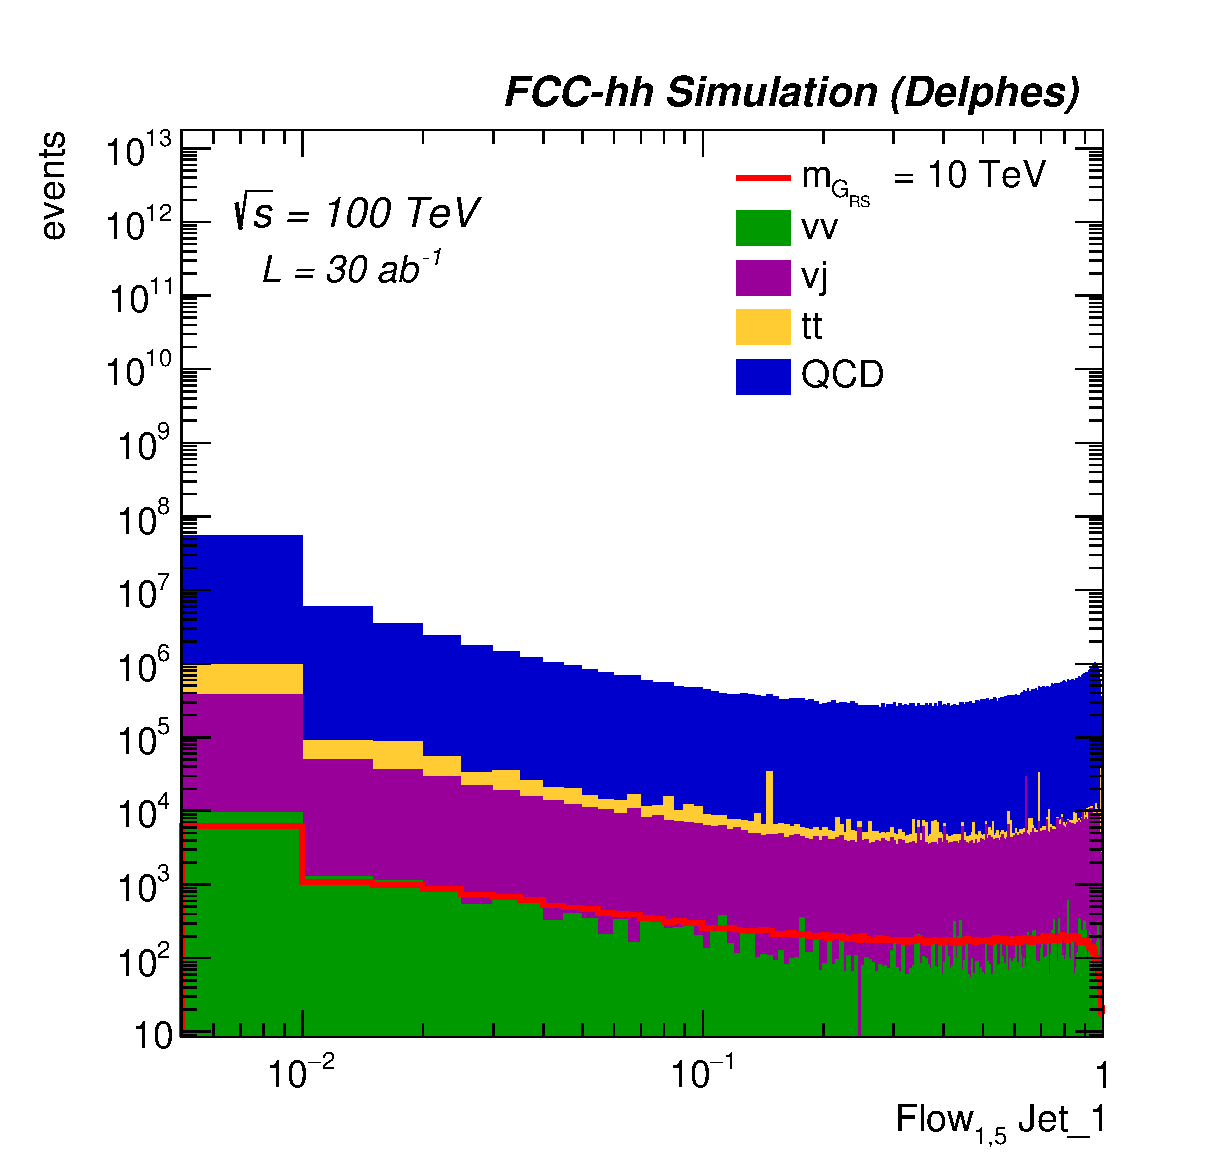
\includegraphics[width=0.45\textwidth]{Fig/TMVA/Jet1_Flow15_sel0_nostack_logx.eps}
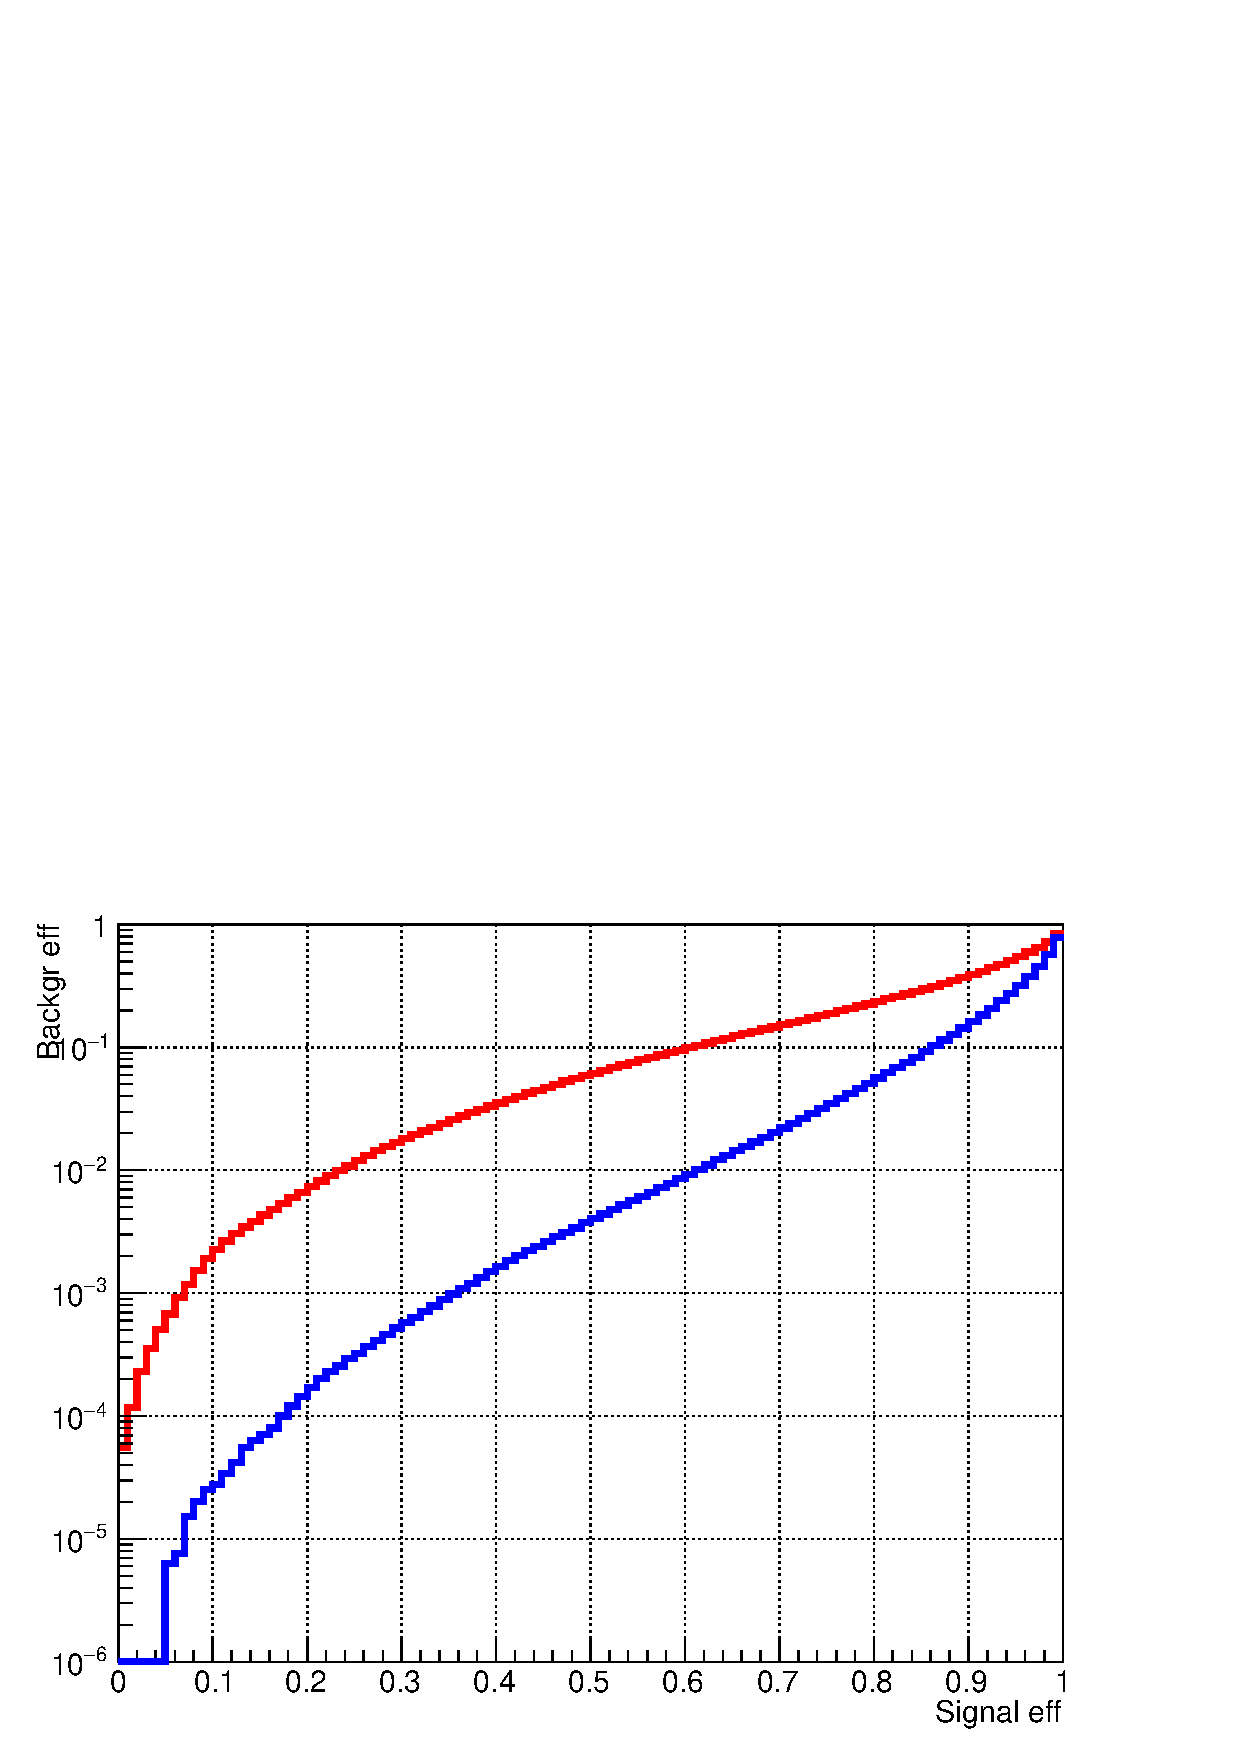
\includegraphics[width=0.45\textwidth,trim={0 0.5cm 0 0},clip]{Fig/TMVA/effQCD_vs_effWhadBlue_thadRed_log.pdf}
\caption{Left: Energy-flow ($E_{F}(1,0.05)$) observable for W and QCD jets. Right: Light jet rejection versus tagging efficiency for the $W$ tagger (blue) and top tagger (red).}
\label{fig:TMVA_final_result}
\end{figure}

%\clearpage
%\newpage

%%%%%%%%%%%%%%%%%%%%%%%%%%%%%%%%%%%%%%%%%%%%%%%%%%%%%
\subsection{Tag Rate Function}
\label{subsec:trf}
The modeling of the backgrounds in the high tagging regimes is a challenging task.
The requirement of $b$ tagging in some MC samples can drastically reduce the available statistics.
This shortage of events that pass the $b$-tagging cut in the signal regime, in conjunction with the large cross section of some of the backgrounds can lead to very spiky templates.
\newline
To overcome this problem the tag rate function (TRF) method is introduced.
By using the TRF method, no event is cut based on its $b$-tagging count, but instead all the events are weighted.
This weight can be interpreted as the probability of the given event to contain the desired number of $b$ jets.
To achieve this, the tagging efficiency (a function of $\eta$, $\pt$ and true jet flavour) was
used to calculate the event weight based on the kinematics and flavour of the jets found in each event.
\newline
Given a jet with $\eta$, $\pt$ and flavour $f$, its tagging probability can be noted as:
\begin{equation*}
	\varepsilon \left(f,|\eta|,\pt\right)
\end{equation*}
\newline
For a given event with $N$ jets, its probability of containing exactly one $b$-tag jet can be computed as:
\begin{equation*}
	P_{=1} = \sum\limits_{i=1}^N \left( \varepsilon_{i} \prod\limits_{i \neq j} \left( 1 - \varepsilon_{j} \right) \right)
\end{equation*}
\newline
In the same way, it can be used to compute the probability for inclusive $b$-tag selections:
\begin{align*}
	P_{=0} &= \prod\limits_{i=1}^N \left( 1 - \varepsilon_{j} \right) \\
	P_{\geq 1} &= 1 - P_{=0}
\end{align*}
\newline
It was verify that the TRF methods agrees well with the direct tagging.

%%%%%%%%%%%%%%%%%%%%%%%%%%%%%%%%%%%%%%%%%%%%%%%%%%%%%
\subsection{Mass spectrum fit}
Despite the fact that very large amount of Monte-Carlo statistic has been simulated in bins of $\hht$
and the usage of techniques to save events with TRF methods,
there are still large statistical fluctuations from high weight events.
In order to reduce this effect, a function is used to fit the background distribution,
\begin{equation}
f(z)=p_1(1-z)^{p_2}z^{p_3}z^{p_{4}logz}
\end{equation}
where $z=m_{jj}/\sqrt{s}$. This fit is used in order to have a smooth shape for the backgrounds, while the normalisation is taken prior to the fit (see figure~\ref{fig:hadronicresonances_nofit}).

\begin{figure}[!htb]\centering
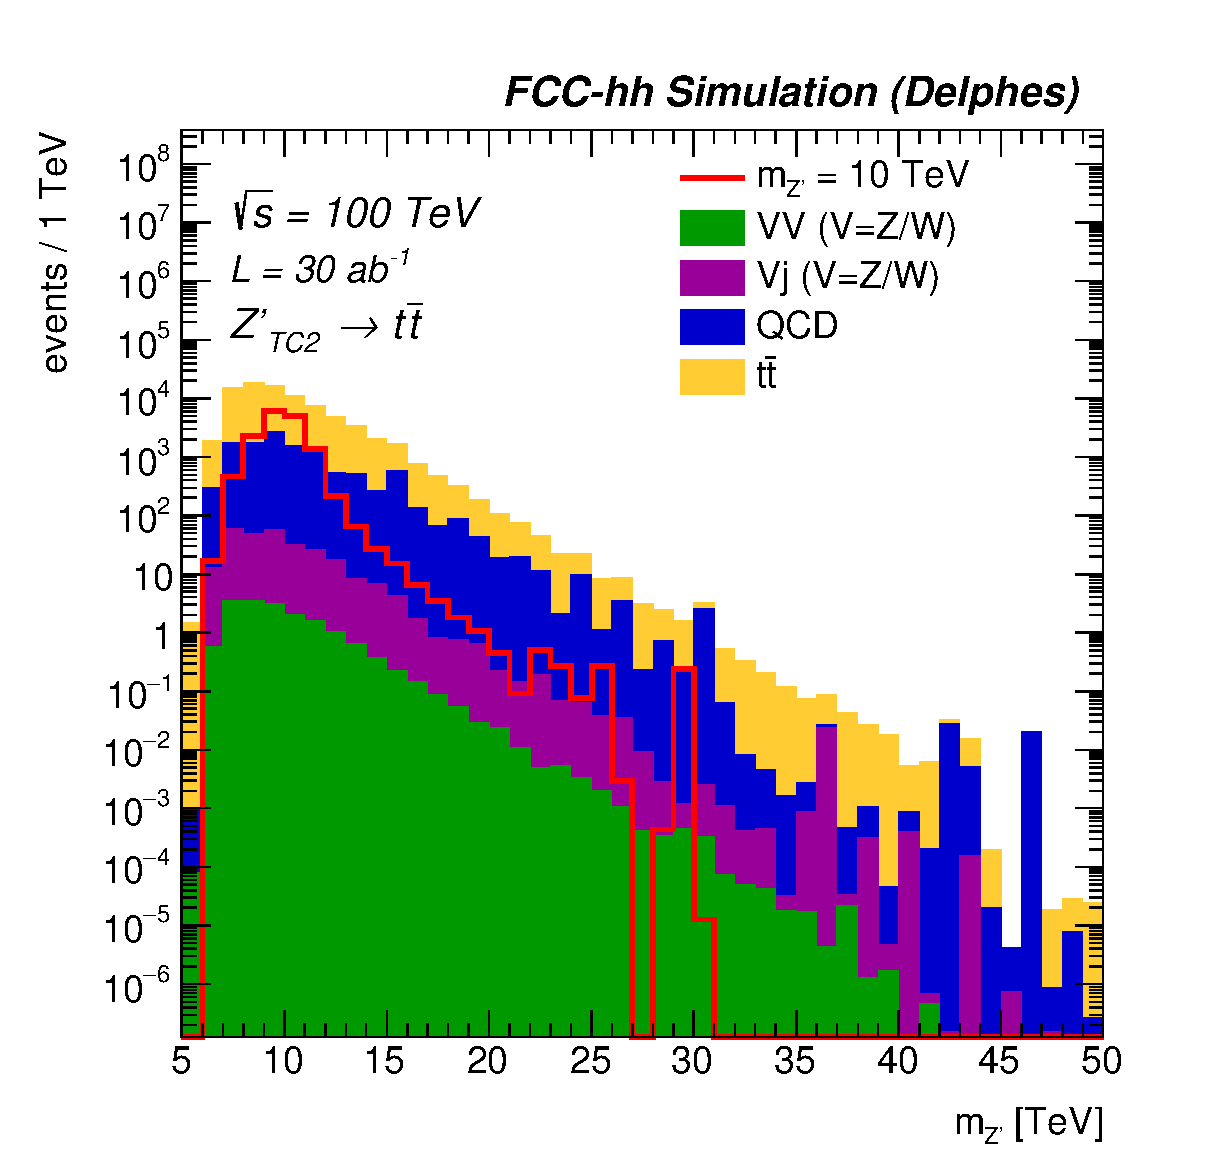
\includegraphics[width=0.45\columnwidth]{Fig/Zptt/Mj1j2_pf08_MetCorr_sel8_nostack_log.eps}
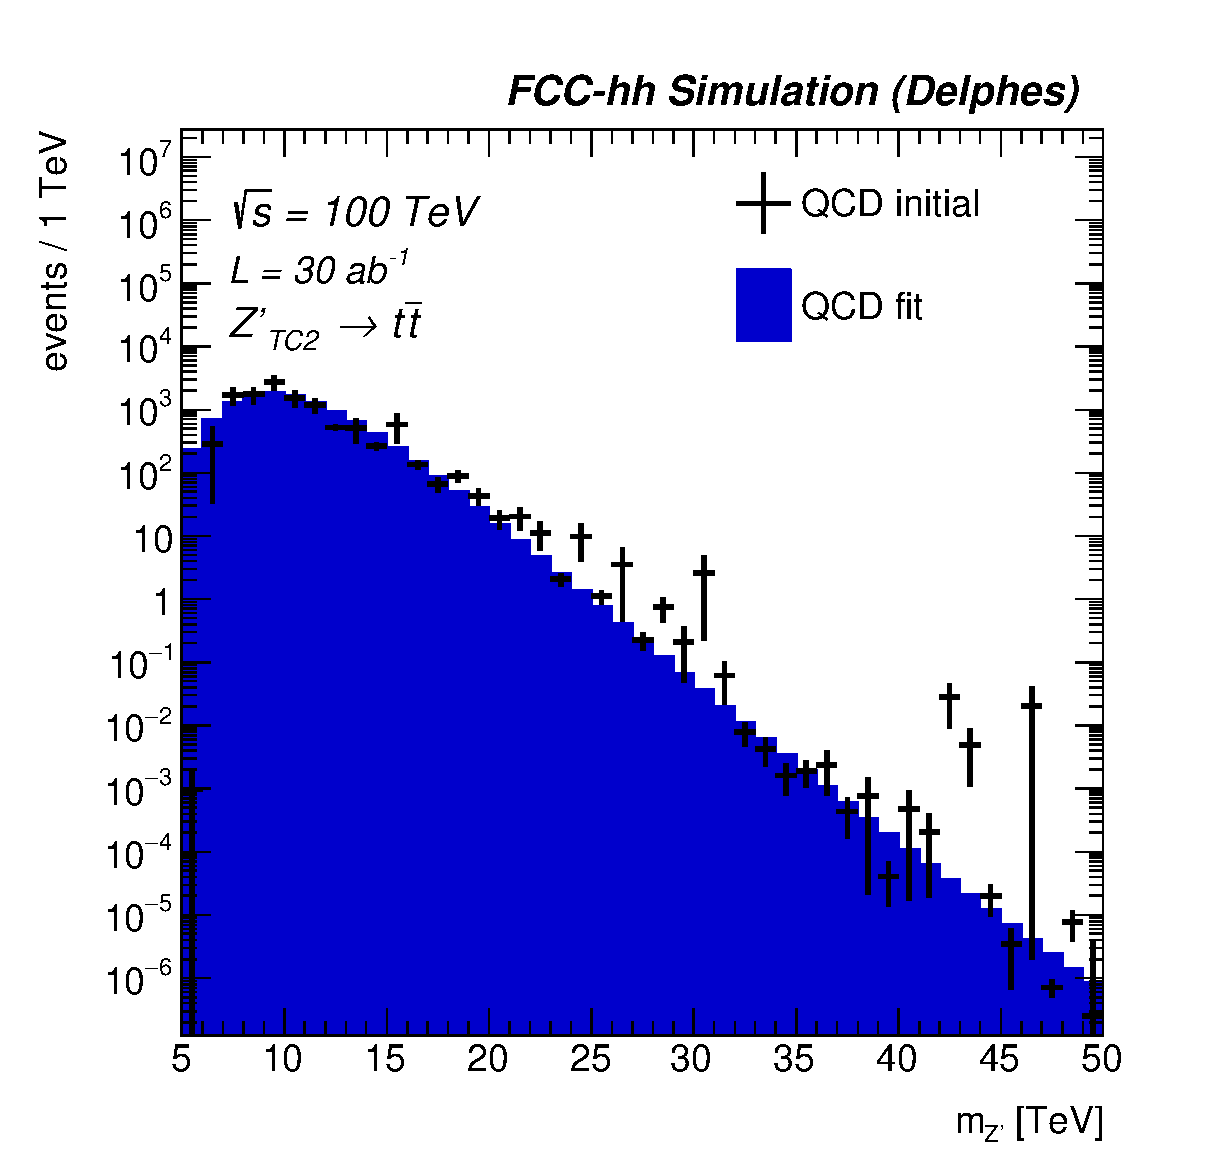
\includegraphics[width=0.45\columnwidth]{Fig/Zptt/Zptt_QCD_sel8_Mj1j2_pf08_MetCorr_fit.eps}
\caption{Invariant mass prior to fit.}
\label{fig:hadronicresonances_nofit}
\end{figure}



\section{Di-lepton channels}
\label{sec:lep}

Models with extended gauge groups often feature additional U(1) symmetries with corresponding heavy spin-1 bosons. These bosons, generally referred to as $\Zp$, would manifest themselves as a narrow resonance in the dilepton mass spectrum. Among these models are those inspired by Grand Unified Theories, motivated by gauge unification or a restoration of the left-right symmetry violated by the weak interaction. Examples include the $\Zp$ bosons of the E6 motivated theories~\cite{London:1986jz,Joglekar:2016yap,Langacker:2008yv,Hewett:1988xc} and Minimal models~\cite{Salvioni:2009mt}. The Sequential Standard Model (SSM)~\cite{Langacker:2008yv} posits a $\ZpSSM$ boson with couplings to fermions that are identical to those of the Standard Model $\Z$ boson.

The decay products of heavy resonances are in the multi-TeV regime and the capability to reconstruct their momentum imposes stringent requirement on the detector design. In particular, reconstructing the track curvature of multi-TeV muons requires excellent position resolution and a large lever arm. In this section, the expected sensitivity is presented for a \Zpll\ (where $\ell=\mathrm{e},\mu$) and \Zptata\ separately.


\subsection{The \ee\ and \mumu final states}
\label{sec:lepee}

Events are required to contain two isolated opposite sign leptons with $\pt > 1$~TeV, $|\eta|$<4 and an invariant mass $\mll > 2.5$~TeV.
Figure~\ref{figure:leptonicresonances:masses} (left and center) shows the invariant mass for a 30~TeV signal for the $ee$ and $\mu\mu$ channels. The mass resolution is better for the ee channel, as expected. , and the yields can be found in Table~\ref{tab:leptonicresonances:yieldsll}.

\MS{distinguish 27 and 100 TeV}

\begin{table}[htbp]
   \centering
\begin{tabular}{|l|r|r|}
  \hline
  \hline
 & ee & $\mu\mu$  \\
  \hline
  Drell-Yan & 206882.9 & 236597.9 \\
  \hline
  $\Zp$ 4~TeV & 1421357.9    & 1598969.4 \\
  $\Zp$ 6~TeV & 349922.4  & 393117.6\\
  $\Zp$ 8~TeV &   115043.5 & 129698.7 \\
  $\Zp$ 10~TeV &  45423.5 & 50873.3 \\
  $\Zp$ 20~TeV &  1192.3 & 1411.5\\
  $\Zp$ 30~TeV &  88.2 & 107.6\\
  $\Zp$ 40~TeV &  11.7 & 14.1 \\
  $\Zp$ 50~TeV &  3.2 & 3.7\\
  \hline
  \hline
\end{tabular}
  \caption{Expected number of events for the \Zpee\ and \Zpmumu\ analysis after the full event selection for the various \Zp\ mass hypotheses \MS{100 TeV}}
  \label{tab:leptonicresonances:yieldsll}
\end{table}

\begin{figure}[!htb]
  \centering
  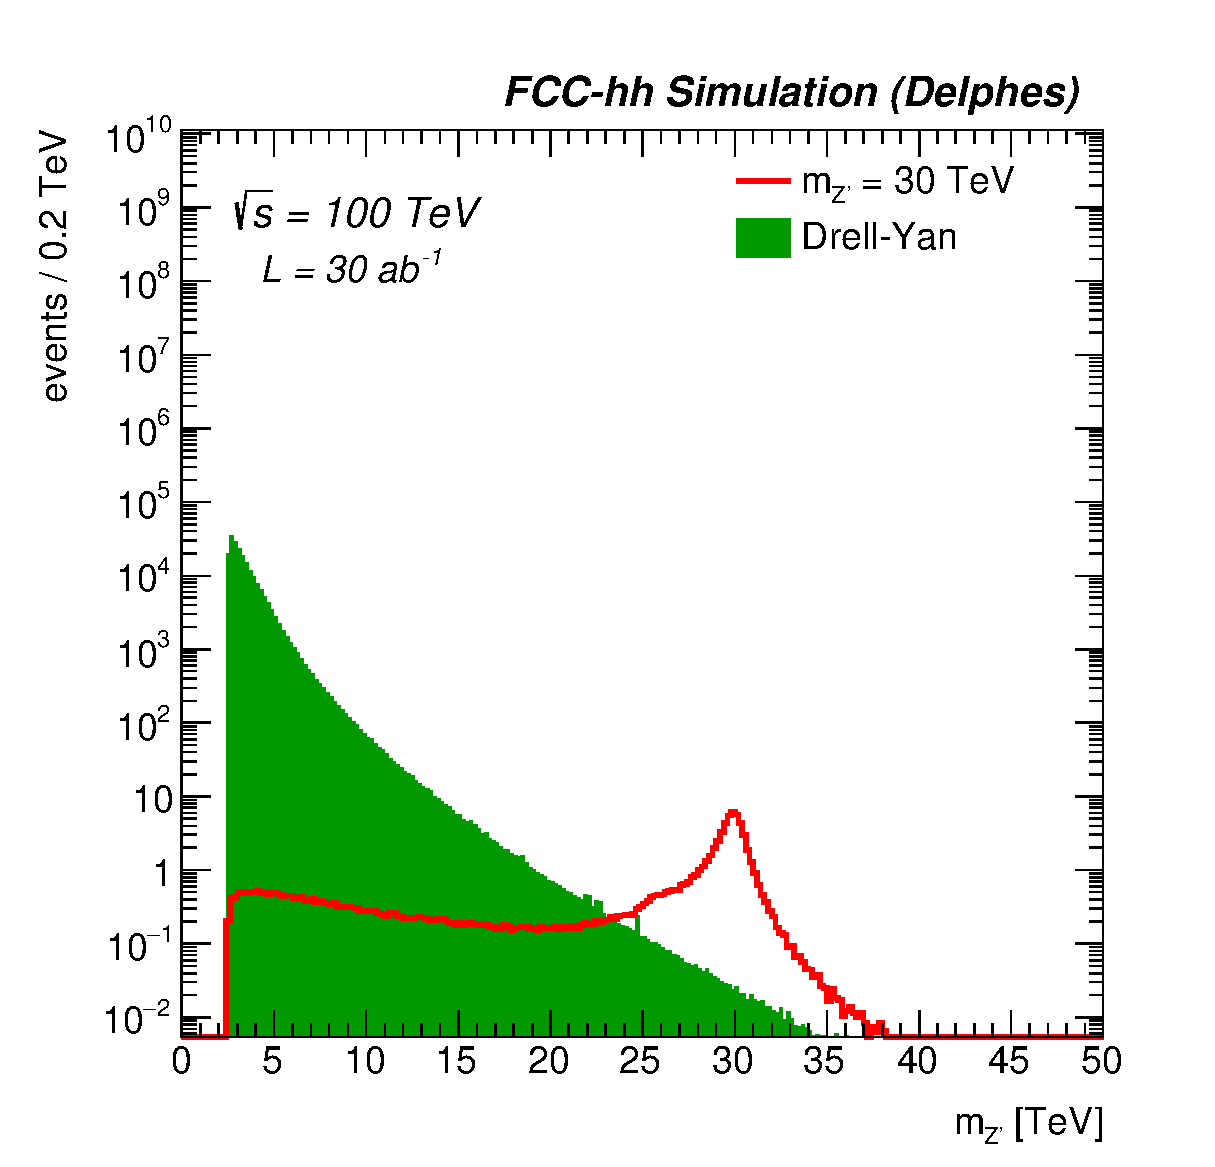
\includegraphics[width=0.32\columnwidth]{Fig/mzp_sel0_nostack_log_ee.eps}
  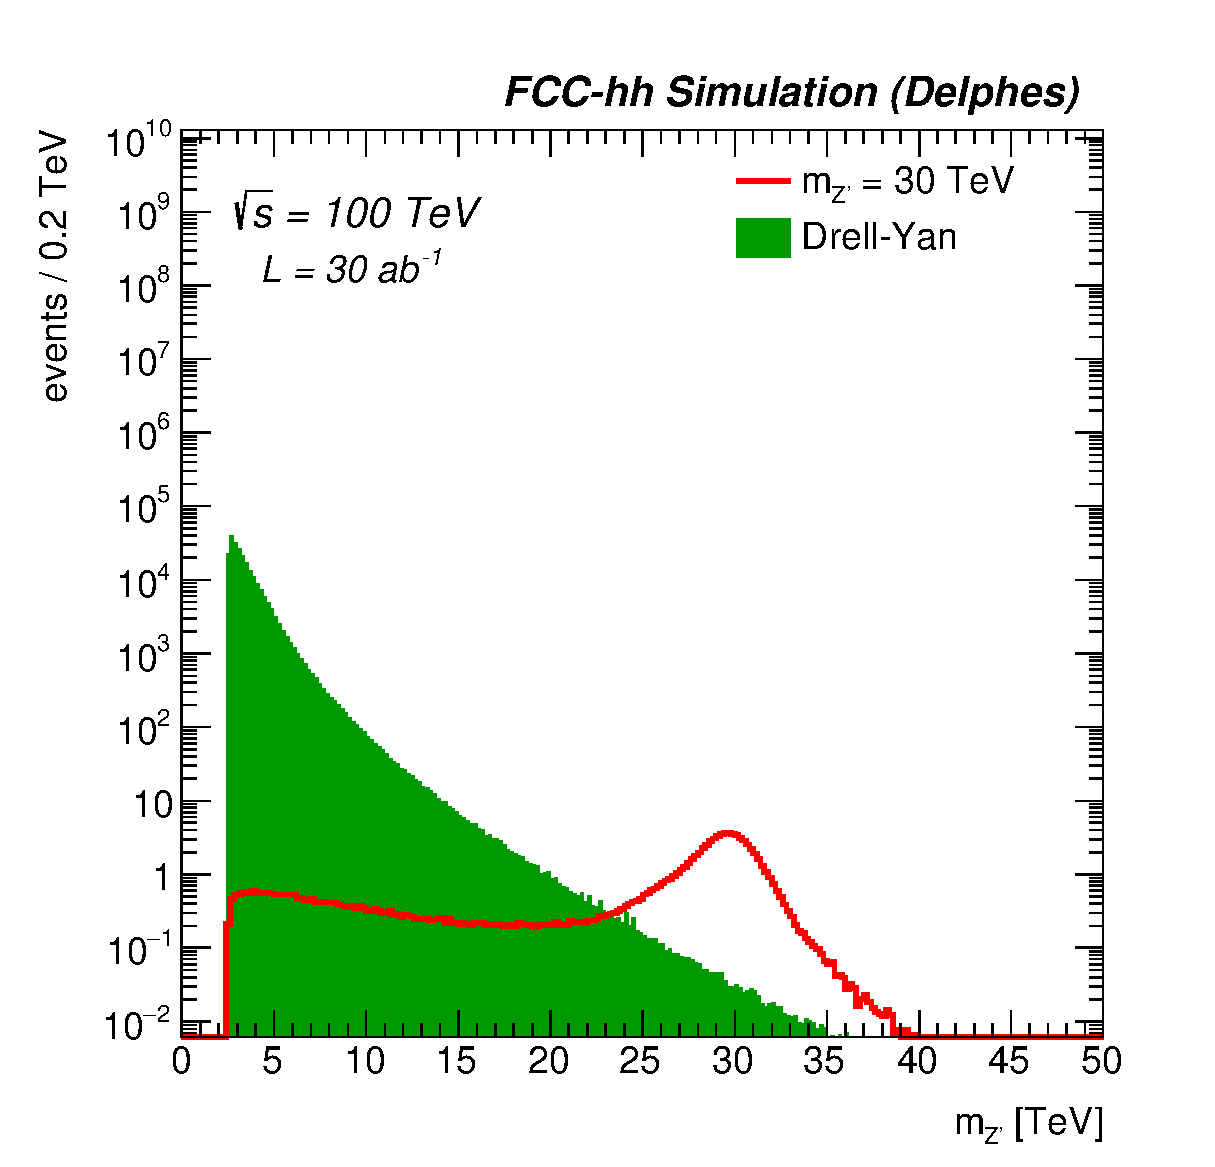
\includegraphics[width=0.32\columnwidth]{Fig/mzp_sel0_nostack_log_mm.eps}
  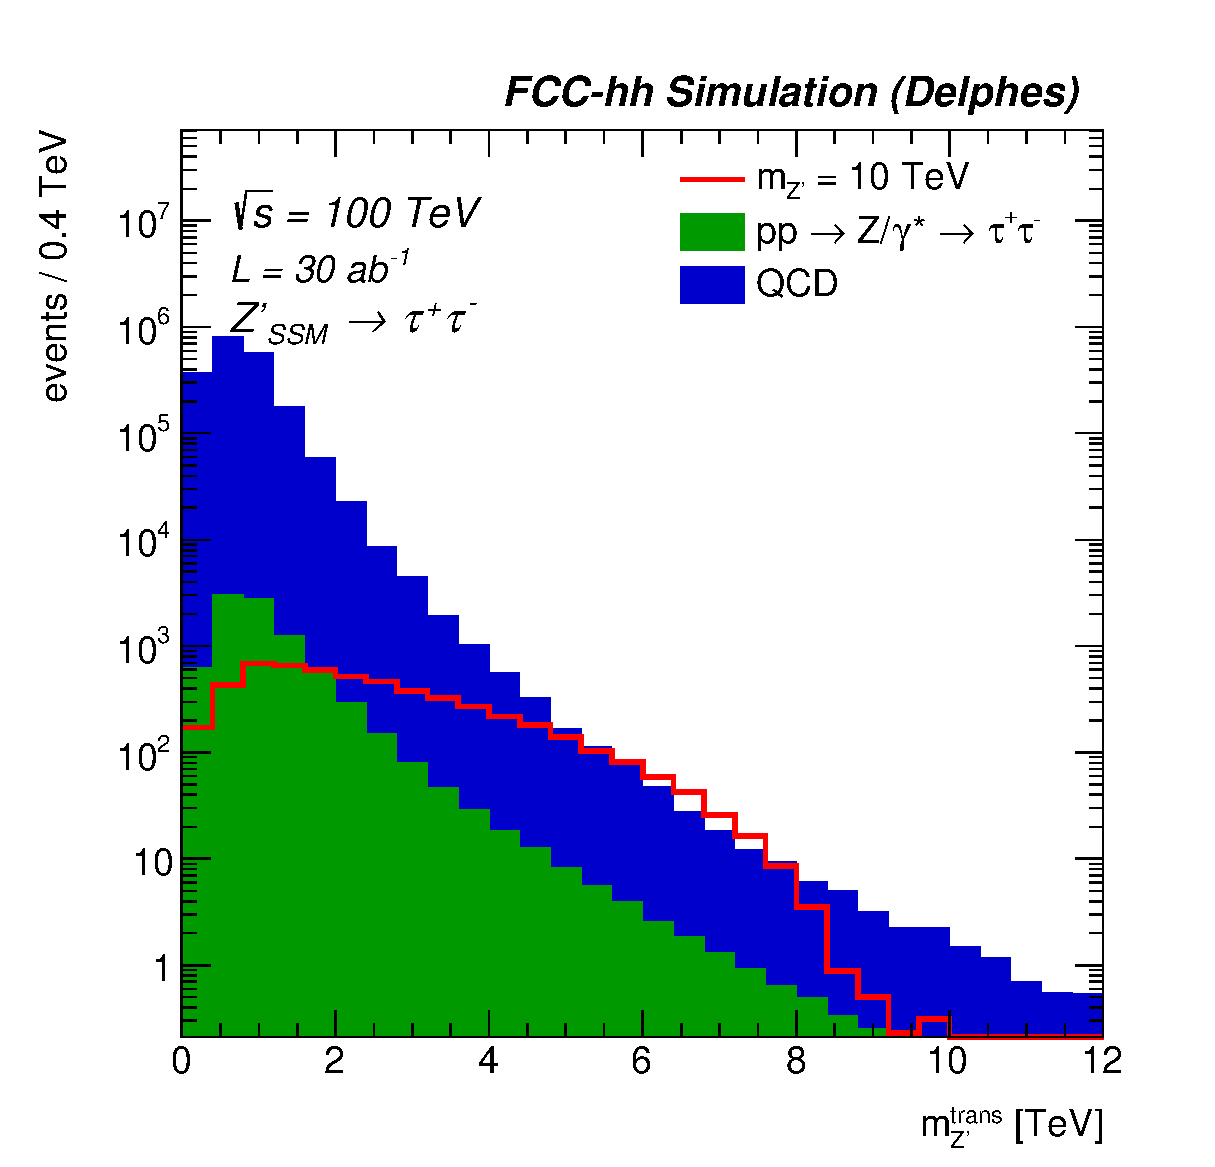
\includegraphics[width=0.32\columnwidth]{Fig/mt_finalsel_nostack_log.eps}
  \caption{Left, center: Invariant mass for a 30~TeV signal after full event selection for ee channel (left) and $\mu\mu$ channel (center). Right: Transverse mass for a 10~TeV signal after full event selection for the $\tau\tau$ channel.\MS{maybe split \tautau\ and \ellell}}
  \label{figure:leptonicresonances:masses}
\end{figure}

Hypothesis testing is performed using a modified frequentist method based on a profile likelihood that takes into account the systematic uncertainties as nuisance parameters that are fitted to the expected Monte-Carlo\MS{mention here that will be sued for all channels, or maybe say in a common section appearing before}. For the $ee$ and $\mu\mu$ analyses, the di-lepton invariant mass is used as the discriminant, while for the $\tau\tau$ channel the transverse mass is used. A 50\% uncertainty on the background normalisation is assumed.

Figure~\ref{figure:leptonicresonances:resultsll} shows the exclusion limit obtained \intlumifcc\ of data for the ee alone (top left), $\mu\mu$ alone (top right) and combination of (ee,$\mu\mu$) channels (bottom left). Figure~\ref{figure:leptonicresonances:resultsll} (bottom right) shows the integrated luminosity required to reach a $5\sigma$ discovery for the leptonic resonances as a function of the mass of the heavy resonance. The \Zpee\ and \Zpmumu\ channel display very similar performance, due to the low background rates. We conclude therefore that the reference detector design features near to optimal performance for searches involving high \pt\ muon final states.

The discovery potential for high mass resonances decaying to $ee$, $\mu\mu$ has been studied using as a benchmark the \ZpSSM\ model. The very large centre of mass energy provides a correspondingly large mass reach. For the $ee$ and $\mu\mu$ cases masses up to 42~TeV can be excluded or discovered.


\begin{figure}[!htb]
  \centering
  \includegraphics[width=0.33\columnwidth]{Fig/lim_Zprime_ee_fcc_v02_allxs.eps}
  \includegraphics[width=0.33\columnwidth]{Fig/lim_Zprime_mumu_fcc_v02_allxs.eps}
  \includegraphics[width=0.33\columnwidth]{Fig/lim_Zprime_ll_fcc_v02_allxs.eps}
  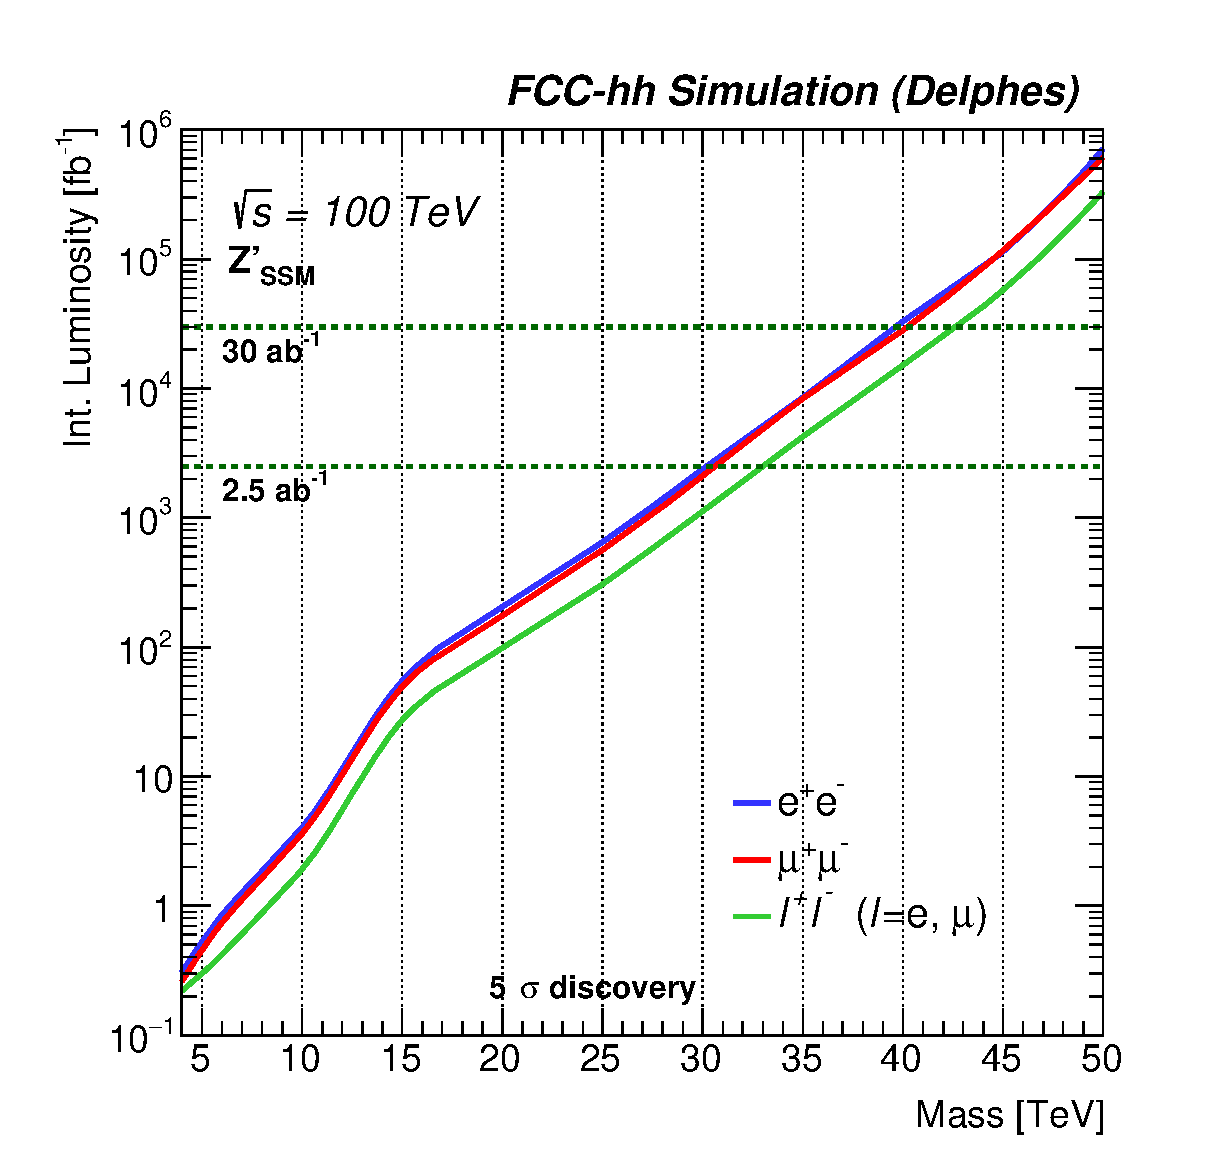
\includegraphics[width=0.33\columnwidth]{Fig/DiscoveryPotential_ll_comb_rootStyle.eps}
  \caption{Limit versus mass for the di-lepton (ee,$\mu\mu$) channel (left) and luminosity for a $5\sigma$ discovery (right) comparing ee,$\mu\mu$ and combined channels. }
  \label{figure:leptonicresonances:resultsll}
\end{figure}



\subsection{The \tautau\ final state}
\label{sec:leptautau}

The di-$\tau$ event selection requires two jets with $p_{T} > 0.5$>~TeV and $|\eta|<2.5$ identified as $\tau$'s. To ensure no overlap between the $\ell$ and $\tau$ final states, jets containing leptons with $\pt > 100$~GeV are vetoed. Finally, requirements of $\Delta \phi(\tau_1, \tau_2)> 2$ and $2.5<\Delta R(\tau_1, \tau_2)<4$ are applied.
Mass dependent cuts applied to maximise the signal to background ratio are summarised in Table~\ref{tab:leptonicresonances:selectiontautau}. Figure~\ref{figure:leptonicresonances:masses} (right) shows the transverse mass~\footnote{the transverse mass is defined as $m_{T}  =  \sqrt{2\ptZp*\met*(1-cos\Delta\phi(\Zp,\met))} $}
of a 10~TeV signal for the $\tau\tau$ channel. Several proxies for the true resonance mass have been tested, such as the invariant mass of the two taus, with and without correction for the missing energy. The transverse mass provided the best sensitivity and was therefore used to set limits and determine the discovery reach.

\MS{distinguish 27 and 100 TeV}

\begin{table}[htbp]
   \centering
\begin{tabular}{|l|l|c|r|}
  \hline
  \hline
   $\Zp$ mass [TeV] &  $\Delta \phi(\tau_1, \tau_2)$&  $\Delta R(\tau_1, \tau_2)$ & $\met$\\
  \hline
  $4-8$ & > 2.4 & > 2.5 and < 3.5 & > 400 GeV\\
  $10$ & > 2.4 & > 2.7 and < 4 & > 300 GeV\\
  $12-14$ & > 2.6 & > 2.7 and < 4 & > 300 GeV\\
  $16-18$ & > 2.7 & > 2.7 and < 4 & > 300 GeV\\
  $>18$ & > 2.8 & > 3 and < 4 & > 300 GeV\\
  \hline
  \hline
  \end{tabular}
  \caption{List of mass dependent cuts optimised to maximise the sensitivity for the \Zptata\ search.}
  \label{tab:leptonicresonances:selectiontautau}
\end{table}

Figure~\ref{figure:leptonicresonances:resultstautau} shows the exclusion limits for 30 ab$^{-1}$ of data (left) and the required integrated luminosity
versus mass to reach a $5\sigma$ discovery (right) for the di-tau resonances.

The discovery potential for high mass resonances decaying to $\tau\tau$ has been studied using as a benchmark the \ZpSSM\ model. The very large centre of mass energy provides a correspondingly large mass reach. Heavy resonance decaying to $\tau$ leptons reconstructed in the hadronic decay mode are more challenging, but we would be able to probe massses up to 18~TeV.

\begin{figure}[!htb]
  \centering
  \includegraphics[width=0.33\columnwidth]{Fig/lim_Zprime_tautau_fcc_v02_allxs.eps}
  \includegraphics[width=0.33\columnwidth]{Fig/DiscoveryPotential_tautau_rootStyle.eps}
  \caption{Limit versus mass for the di-tau channel (left) and luminosity for a $5\sigma$ discovery (right). }
  \label{figure:leptonicresonances:resultstautau}
\end{figure}


The discovery potential for resonances considered in FCC-hh scenario are summarised in Figure~\ref{figure:resonances100:summary}.

\begin{figure}[!htb]
  \centering
  \includegraphics[width=0.90\columnwidth]{Fig/summaryDisco_onlyFCChh.pdf}
  \caption{Summary of a $5\sigma$ discovery reach as a function of the resonance mass for different luminosity scenario of FCC-hh.}
  \label{figure:resonances100:summary}
\end{figure}



\section{Hadronic final states}
\label{sec:hadronic}

Many models of beyond the SM (BSM) physics predict additional particles with masses at the TeV scale. The presence of new resonant states~\cite{Harris:2011bh,Boelaert:2009jm,Lee:1973iz,Branco:2011iw,Hill:1994hp,Kaplan:1983sm,Bellazzini:2014yua,Randall:1999ee,Pomarol:1999ad,Davoudiasl:1999tf} decaying to two highly boosted particles decaying hadronically could be observed as an excess in the QCD dijet distribution. We focus here on three specific benchmark models: a \ZpSSM~\cite{Langacker:2008yv}, a Randall-Sundrum graviton~\cite{Randall:1999ee}, and an excited quark resonance~\cite{Baur:1987ga,Baur:1989kv}. We study the sensitivity in the following decay using hadronic decay modes: \Zptt, \rsg\ and \qjj.

The decay products are typically in the multi-TeV regime and their reconstruction imposes stringent requirement on the detector design. Precise jet energy resolution requires full longitudinal shower containment. Highly boosted top quarks and $W$ bosons decay into highly collimated jets that need to  be disentangled from standard QCD jets by studying their substructure. High discrimination power and sensitivity for these searches at such extreme energies, requires excellent granularity both in the tracking detectors and calorimeters.


\subsection{The \jj\ final state}
\label{sec:hadjj}

Jets are clustered using particle-flow candidates with the anti-$k_T$~\cite{Cacciari:2008gp} algorithm with parameter R=0.4. We require at least two jets with $\pt$>3~TeV and $|\eta<3|$ and the rapidity difference between the two leading jets to be small, $\Delta(\eta)<1.5$ as di-jet events will tend to be more central. The dijet invariant mass of the \qjj\ signal for $m_Q^{*}$ and QCD contributions after the full event selection is shown in Figure~\ref{figure:hadronicresonances:ttsel08} (left).


\subsection{The \ttbar\ final state}
\label{sec:hadtt}

As track jets are better able to resolve the jet sub-structure compared to particle-flow jets, the jet selection for the \rsg\ and \Zptt\ searches using track jets. As no lepton veto is applied, there is also some acceptance for leptonic decays. The sensitivity to semi-leptonic $WW$ or \ttbar\ decays is enhanced by adding the $\metvec$ vector to the closest jet 4-momentum (among the to leading jets).

We require two jets with a $\pt$>3~TeV and $|\eta<3|$ and $\Delta(\eta)<2.4$. Both jets must either be $W$ or top tagged (section~\ref{subsec:mvatagger}) by requiring multivariate tagger > 0.15. Both high-\pt\ jets must be $b$-tagged for the \Zptt\ analysis. Finally, to further reject QCD, we require for both jets $m_{SD}>40$~GeV. In Figure~\ref{figure:hadronicresonances:ttsel08} we show the di-jet invariant mass distribution after the final cuts for the \rsg\ (center) and \Zptt\ (right) analyses respectively.

\begin{figure}[!htb]
  \centering
  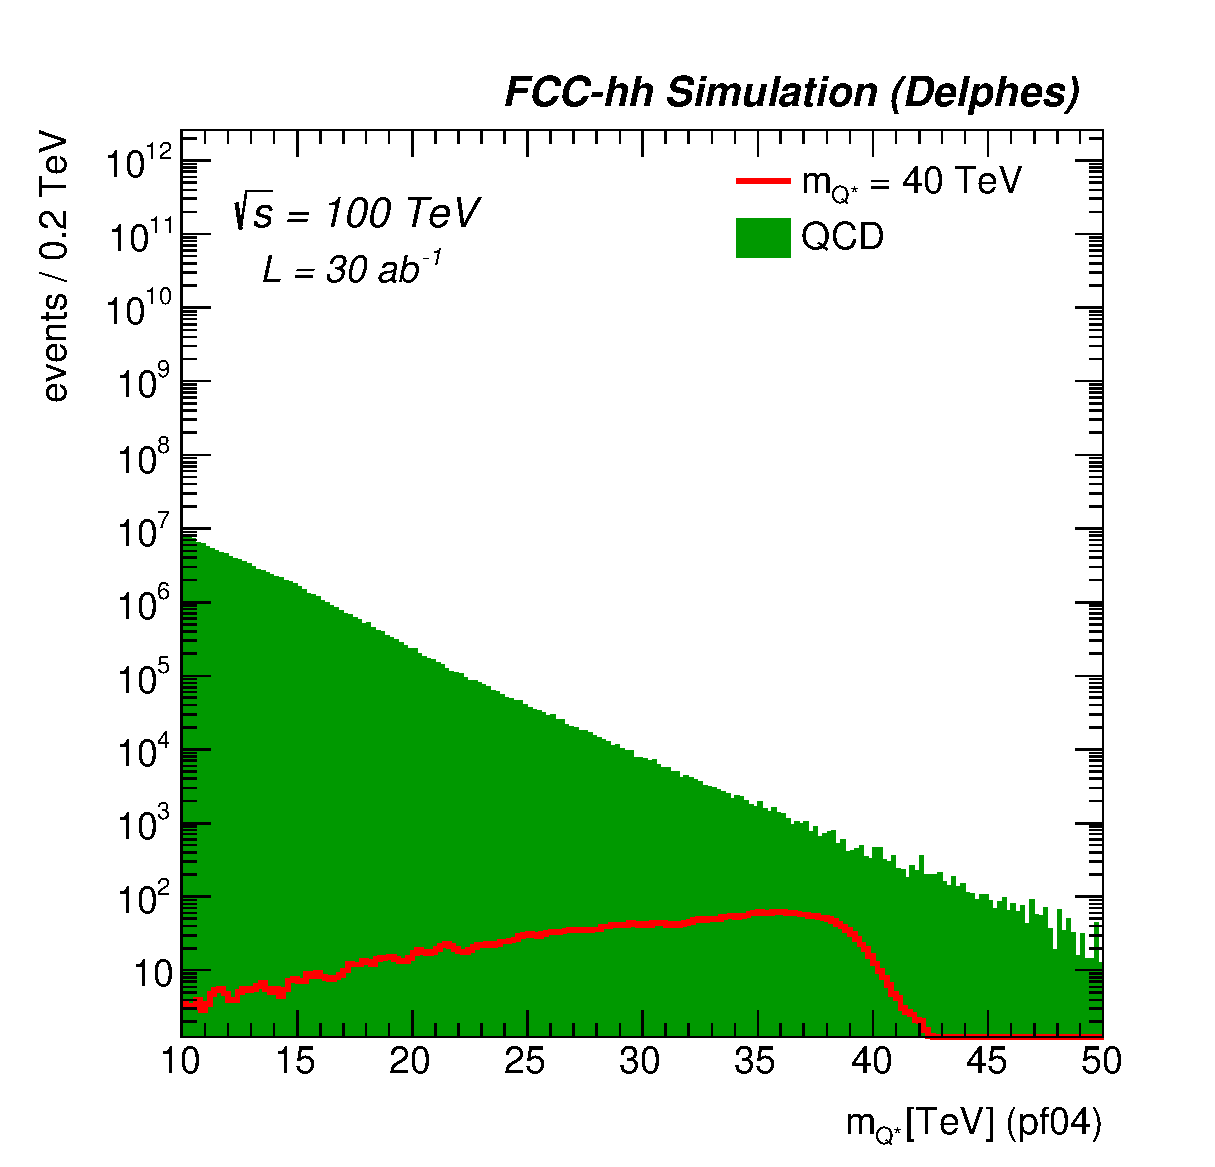
\includegraphics[width=0.32\columnwidth]{Fig/Mj1j2_pf04_sel1_nostack_log.eps}
  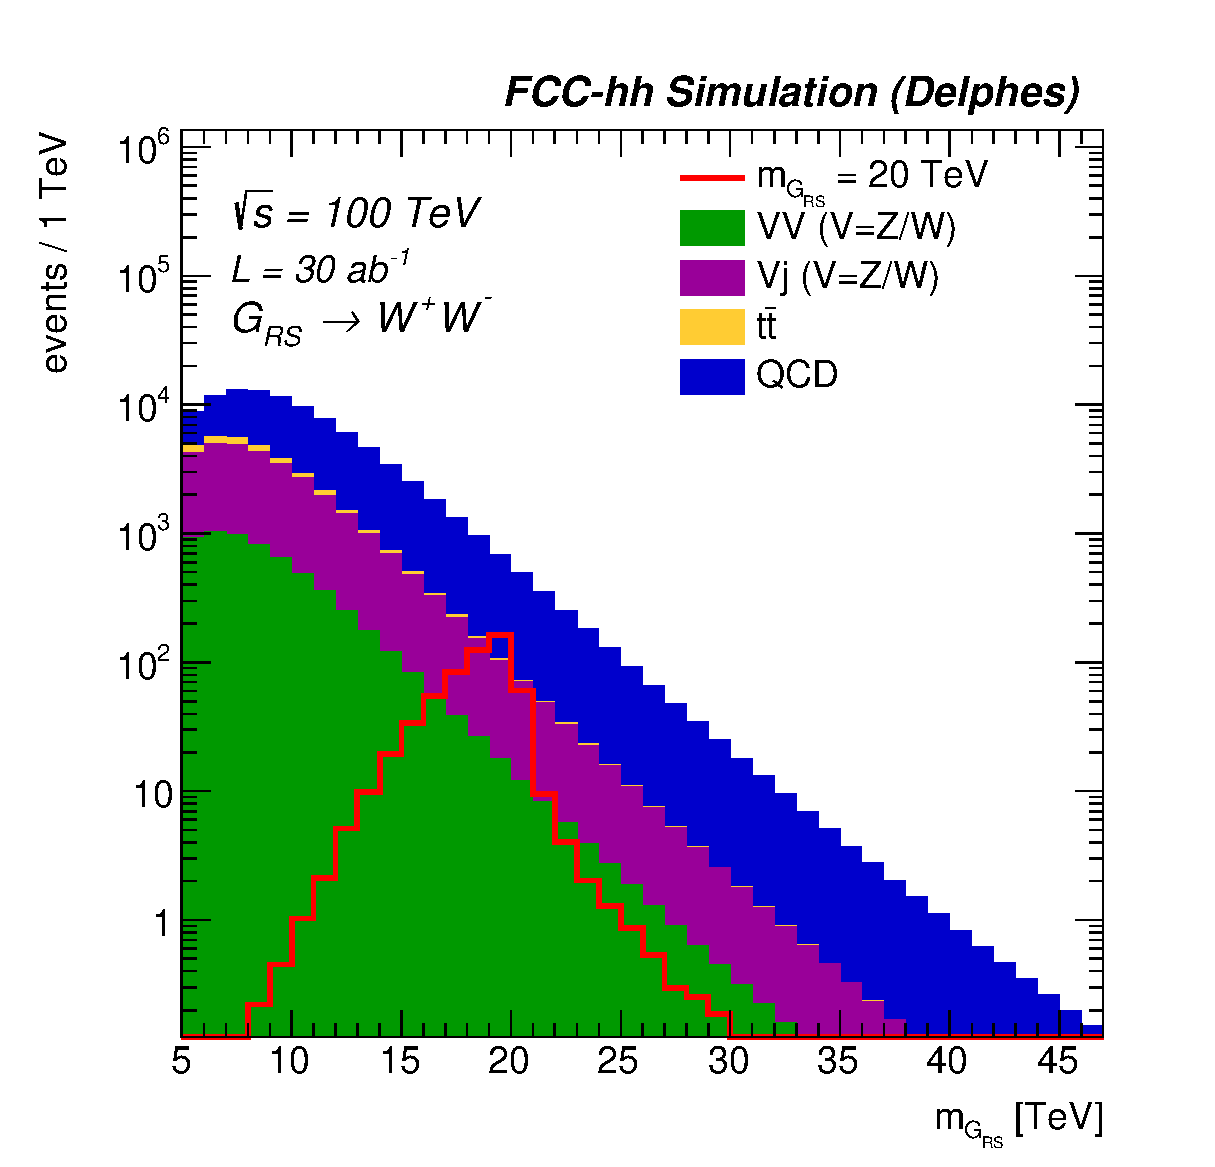
\includegraphics[width=0.32\columnwidth]{Fig/Mj1j2_pf08_fit_sel4_nostack_log.eps}
  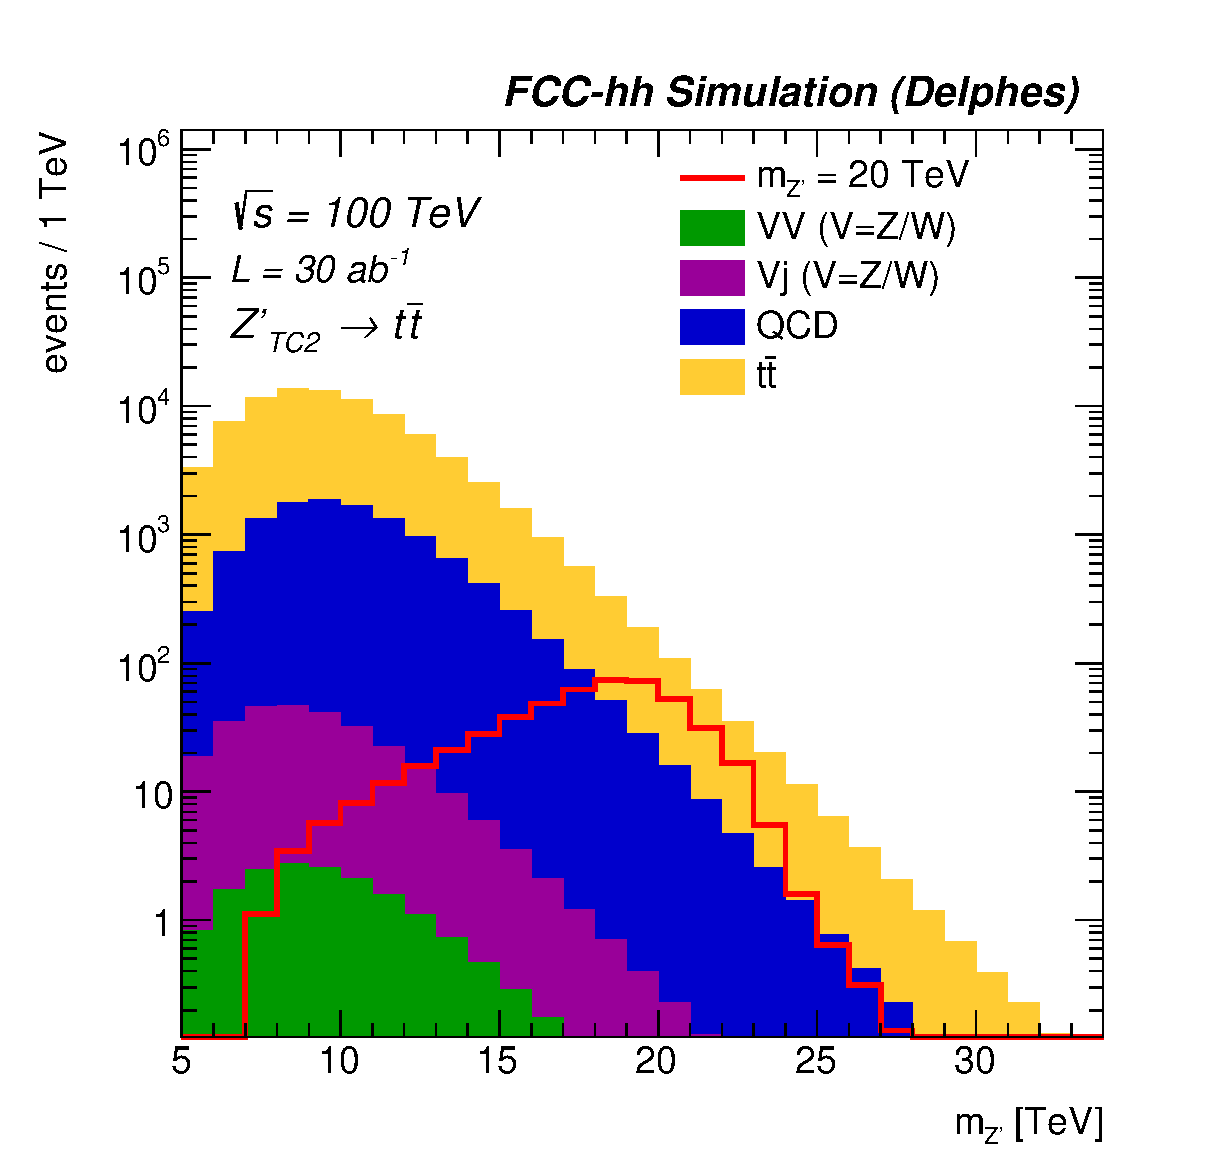
\includegraphics[width=0.32\columnwidth]{Fig/Mj1j2_pf08_MetCorr_fit_sel8_nostack_log.eps}
  \caption{Invariant mass distribution of the two leading jets for the pre-selection (left) and full selection (right) for a 40~TeV signal for the \qjj\ (left), and a 20~TeV signal for \rsg\ (center) and \Zptt\ (right) analyses.\MS{need editing / style}}
  \label{figure:hadronicresonances:ttsel08}
\end{figure}

\begin{table}[htbp]
   \centering
\begin{tabular}{|c|c|c|c|c|c|c|c|c|}
  \hline
  \hline
  & \multicolumn{2}{c|}{di-jet}  & \multicolumn{2}{c|}{$\ttbar$} & \multicolumn{2}{c|}{WW} \\
  \cline{2-7}

 & pre-sel & final-sel  & pre-sel & final-sel & pre-sel & final-sel\\
  \hline
  di-jet & 385555434 &  373661126 &  154855591 & 11439.8&  154856148 & 64484\\
  $\ttbar$ & - & - & 1114779 & 74193.6 &  1114779 & 3185\\
  di-bosons & - & - &  41820 &  17.1 &  41820 & 6092\\
  boson+jet & - & - & 1610472 & 264.1&  1610472 & 25377\\
  \hline
  total bkg  &  385555434& 373661126& 157622662 & 85914 & 154856148 & 99137\\
  \hline
  10~TeV &  - & - &  101529 & 15601 &  47853 & 15745\\
  20~TeV &   1253072 &  1239813& 7774 & 500.6 & 1282 & 578\\
  30~TeV &  69922 &  67488 & 485.2 & 13.2 &  61.4 & 30.1 \\
  40~TeV &  4589 &  4373 & - & - & - & -\\
  \hline
  \hline
\end{tabular}
  \caption{Yields for the di-jet, $\ttbar$ and WW analyses after pre and final selection.}
  \label{tab:hadronicresonances:yields}
\end{table}

\subsection{The \ww\ final state}
\label{sec:hadww}

Hypothesis testing is performed using a modified frequentist method based on a profile likelihood fit that takes into account the systematic uncertainties as nuisance parameters. The di-jet invariant mass is used as a discriminant. In order to reduce large statistical fluctuations from high Monte Carlo weight events, we parameterize the background invariant mass distribution with the following function (conservatively assuming 50\% uncertainty on the background normalisation) $f(z)=p_1(1-z)^{p_2}z^{p_3}z^{p_{4}logz}$, where $z=m_{jj}/\sqrt{s}$.

The expected exclusion limits at 95\% CL are shown in Figures~\ref{figure:hadronicresonances:limits} and~\ref{figure:hadronicresonances:resultsjj}. For the \qjj\ masses up to 40~TeV could be discovered with \intlumifcc. Reconstructing Heavy resonances decaying to $WW$ and \ttbar\ is more challenging and requires the use of novel approaches to boosted object tagging to reduce the backgrounds. The reach for \Zptt\ (in TC2 models) and \rsg\ is 24~TeV and 22~TeV respectively and it is possible to discover a $Z^{\prime}_{SSM} \rightarrow \ttbar$ up to $m_{Z}=18$~TeV.

\begin{figure}[!htb]
  \centering
  \includegraphics[width=0.30\columnwidth]{Fig/lim_Qstar_jj_fcc_v02.eps}
  \includegraphics[width=0.30\columnwidth]{Fig/lim_RSGraviton_ww_fcc_v02.eps}
  \includegraphics[width=0.30\columnwidth]{Fig/lim_Zprime_tt_fcc_v02.eps}
  \caption{Exclusion limit at 95\% CL versus heavy resonance mass decaying into di-jet (left), WW (center), \ttbar\ (right).}
  \label{figure:hadronicresonances:limits}
\end{figure}

\begin{figure}[!htb]
  \centering
  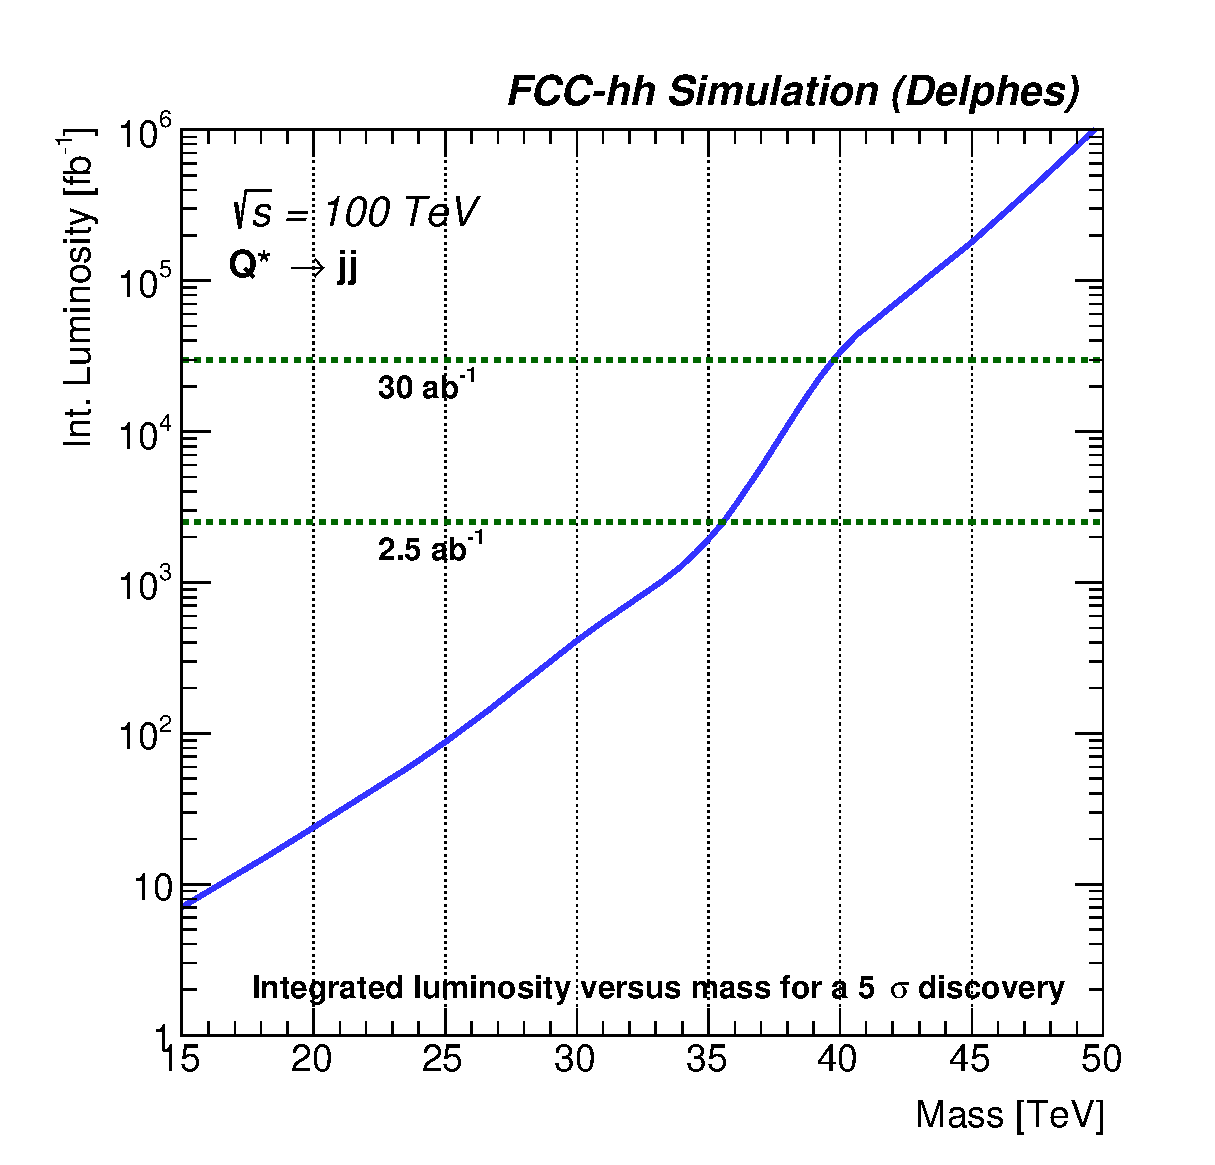
\includegraphics[width=0.30\columnwidth]{Fig/DiscoveryPotential_jj_rootStyle.eps}
  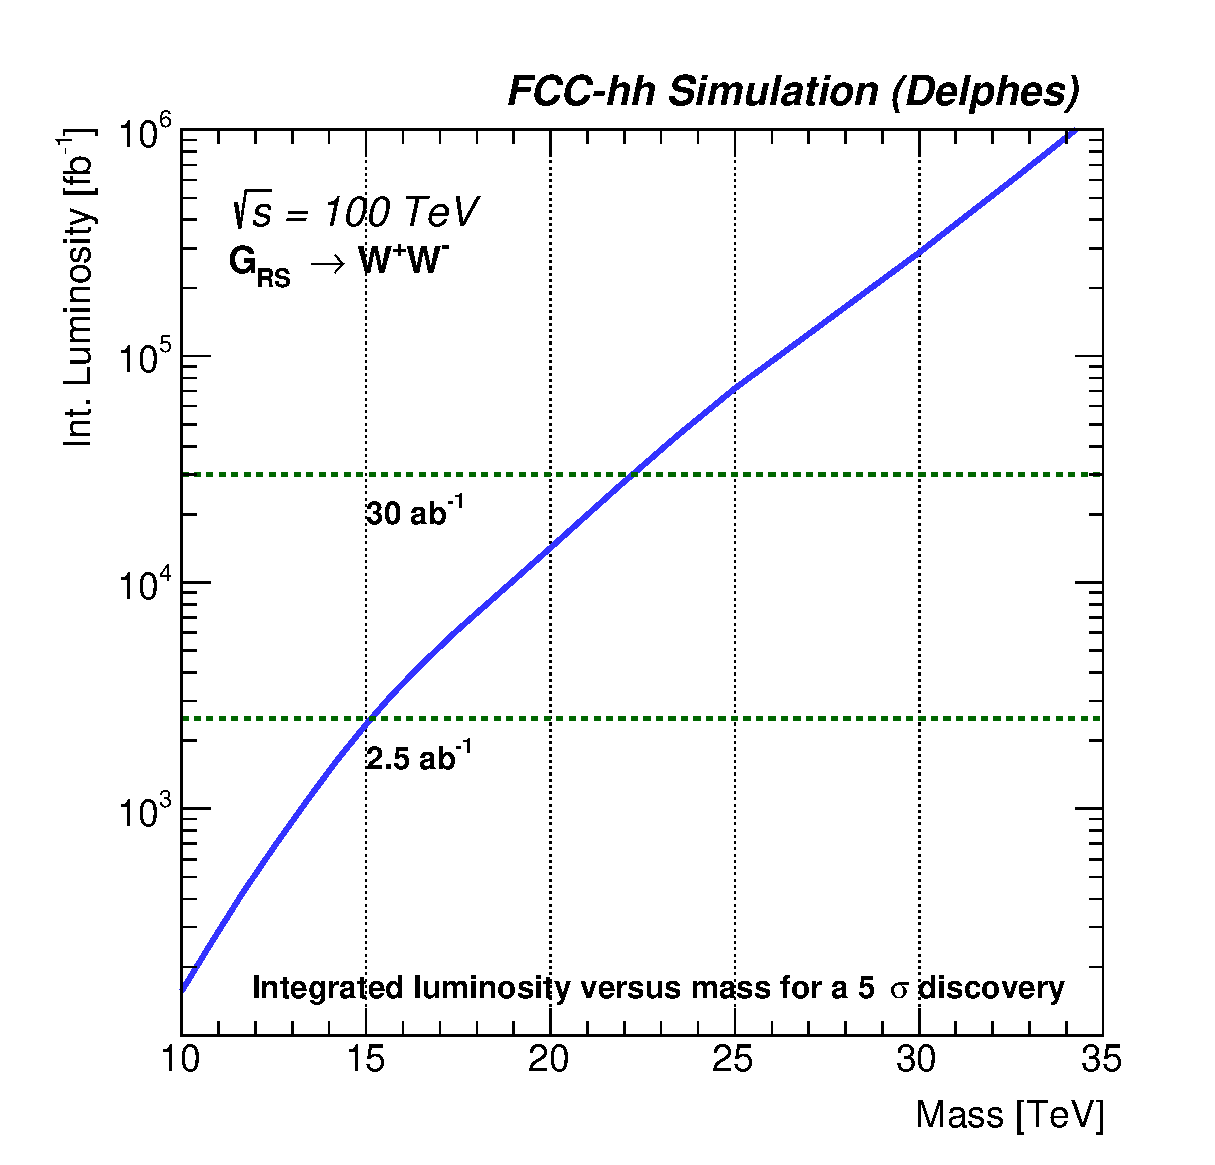
\includegraphics[width=0.30\columnwidth]{Fig/DiscoveryPotential_ww_tagger_rootStyle.eps}
  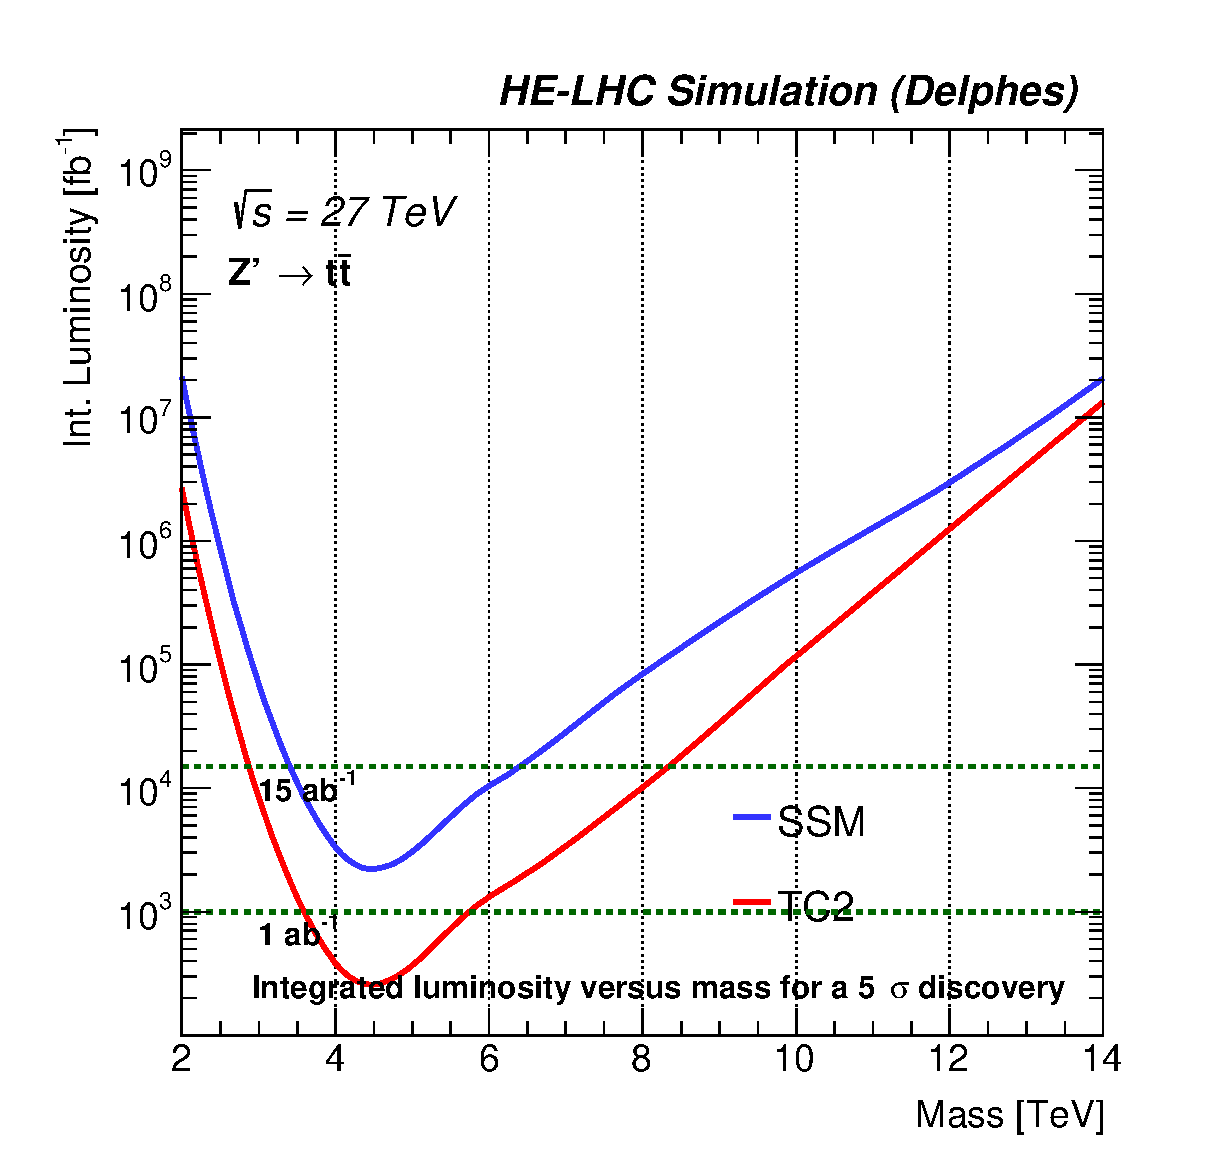
\includegraphics[width=0.30\columnwidth]{Fig/DiscoveryPotential_tt_SSM_TC2_tagger_TRFbtag_rootStyle.eps}
  \caption{Integrated luminosity for a $5\sigma$ discovery as a function of the heavy resonance mass decaying into di-jet (left), WW (center), \ttbar\ (right).}
  \label{figure:hadronicresonances:resultsjj}
\end{figure}

\section{Characterisation of a Z' discovery}
\label{sec:zprimedisc}

\MS{dump directly version that is the YR here.}

\section{Flavour anomaly inspired Z' models sensitivity at the FCC-hh}
\label{sec:zprimeflav}

\MS{completely missing this section}

\section{Conclusion}
\label{sec:conc}

This note presents preliminary studies of a search for $\Zp$
bosons decaying into two electrons or muons in the FCC context. The expected number
of signal and background events have been estimated from simulated truth level information
after applying smearing functions to mimic the FCC detector response.
Using a cut-based analysis and assuming simplistic systematic uncertainties, $\ZpSSM$
masses below 40 $\TeV$ can be excluded at 95$\%$ C.L.
using 30 $\afb{}$ of data.

\appendix
\section{Some title}
Please always give a title also for appendices.





\acknowledgments

This is the most common positions for acknowledgments. A macro is
available to maintain the same layout and spelling of the heading.

\paragraph{Note added.} This is also a good position for notes added
after the paper has been written.





% The bibliography will probably be heavily edited during typesetting.
% We'll parse it and, using the arxiv number or the journal data, will
% query inspire, trying to verify the data (this will probalby spot
% eventual typos) and retrive the document DOI and eventual errata.
% We however suggest to always provide author, title and journal data:
% in short all the informations that clearly identify a document.

\bibliographystyle{JHEP}
\bibliography{refs}

% Please avoid comments such as "For a review'', "For some examples",
% "and references therein" or move them in the text. In general,
% please leave only references in the bibliography and move all
% accessory text in footnotes.

% Also, please have only one work for each \bibitem.


\end{document}
